% Preambel mit Einstellungen importieren
\input{preambel}

% Dokumenteninfos importieren
% -------------------------------------------------------
% Daten für die Arbeit
% Wenn hier alles korrekt eingetragen wurde, wird das Titelblatt
% automatisch generiert. D.h. die Datei titelblatt.tex muss nicht mehr
% angepasst werden.

\newcommand{\hsmasprache}{en} % de oder en für Deutsch oder Englisch

% Titel der Arbeit auf Deutsch
\newcommand{\hsmatitelde}{Diskussion der Vor- und Nachteile von auf Microservices basierenden Softwaresystemen}

% Titel der Arbeit auf Englisch
\newcommand{\hsmatitelen}{Are Microservices for You?  \\ Discussing Trade-offs of Microservice-based Software Systems}

% Weitere Informationen zur Arbeit
\newcommand{\hsmaort}{Mannheim}    % Ort
\newcommand{\hsmaautorvname}{Max} % Vorname(n)
\newcommand{\hsmaautornname}{Becker} % Nachname(n)
\newcommand{\hsmadatum}{30.09.2017} % Datum der Abgabe
\newcommand{\hsmajahr}{2017} % Jahr der Abgabe
\newcommand{\hsmafirma}{SAP SE, Walldorf} % Firma bei der die Arbeit durchgeführt wurde
\newcommand{\hsmabetreuer}{Prof. Thomas Smits, Hochschule Mannheim} % Betreuer an der Hochschule
\newcommand{\hsmazweitkorrektor}{Dr. Michele Mancioppi, SAP SE} % Betreuer im Unternehmen oder Zweitkorrektor
\newcommand{\hsmafakultaet}{I} % I für Informatik
\newcommand{\hsmastudiengang}{IM} % IB IMB UIB IM MTB

% Zustimmung zur Veröffentlichung
\setboolean{hsmapublizieren}{true}   % Einer Veröffentlichung wird zugestimmt
\setboolean{hsmasperrvermerk}{false} % Die Arbeit hat keinen Sperrvermerk

% -------------------------------------------------------
% Abstract


% Background factual information
% method, general aim and the specific aim of the study
% summarize methodology
% indicate achievement/result
% indicate implications of the study (Show how the study contributes to knowledge and information in this area) 

%1. Einleitung/Problem
%2. Forschungsziel
%3. Methode
%4. Befunde
%5. Implikationen


% Kurze (maximal halbseitige) Beschreibung, worum es in der Arbeit geht auf Deutsch
\newcommand{\hsmaabstractde}{Microservices sind ein architektureller Ansatz zur Modularisierung von verteilten Softwaresystemen.
Die vorliegende Masterarbeit evaluiert, für welche Typen von Softwaresystemen Microservices ein geeigneter Ansatz sind.
Hierzu werden systematisch ausgewählte Qualitätssze\-narien bewertet.
Das Ergebnis zeigt, dass Microservices gut geeignet sind, um die Zeit von Entwicklung zur Produktion von 
Features in großen Projekten zu verkürzen, hohe Verfügbarkeit in verteilten Systemen zu erreichen und on-demand Ressourcen effizient zu nutzen.
Hingegen sind Microservices eher ungeeignet, wenn die abzubildende Fachdomäne unklar ist, Fähigkeiten zum Entwickeln und Betreiben von verteilten Systemen gering sind oder Daten-/ Transaktionskonsistenz über verschiedene Geschäftsbereiche garantiert werden soll.
}
% Kurze (maximal halbseitige) Beschreibung, worum es in der Arbeit geht auf Englisch

\newcommand{\hsmaabstracten}{The need to innovate large web scale systems faster has brought about microservices, an emerging architectural concept that decouples the life-cycle of components in a distributed software system.
This thesis uses systematically selected quality attribute scenarios to evaluate which types of software systems stand to gain the most from microservices.
Furthermore, it presents a trade-off discussion that can be applied to specific use cases.
As the evaluation shows, microservices should be considered for use cases where high development velocity, high availability in large scale distributed systems and excellent utilization of on-demand hardware are important.
In contrast, one should not consider microservices if the domain of the project is not fully known, team skills concerning designing, developing and operating distributed systems are not high or data need to be consistent across multiple business areas.}

\begin{document}
\frontmatter

% Römische Ziffern für die "Front-Matter"
\setcounter{page}{0}
\changefont{ptm}{m}{n}  % Times New Roman für den Fließtext
\renewcommand{\rmdefault}{ptm}

% Frontpage
\input{frontpage}

% Inhaltsverzeichnis erzeugen
\cleardoublepage
\pdfbookmark{\contentsname}{Contents}
\tableofcontents

% Korrigiert Nummerierung bei mehrseitigem Inhaltsverzeichnis
\cleardoublepage
\newcounter{frontmatterpage}
\setcounter{frontmatterpage}{\value{page}}

% Arabische Zahlen für den Hauptteil
\mainmatter

% Den Hauptteil mit vergrößertem Zeilenabstand setzen
\onehalfspacing

% ------------------------------------------------------------------
% Hauptteil der Arbeit

% maybe turn concrete and abstract way around. Cause in reality you first see the abstract requirements and then decide to tackle it with a practical design.
% On the other hand Hr. Paulus told us that beginning with a practical example helps the understanding

\chapter{Introduction}

\section{Motivation}
\label{intro:motivation}
\begin{chapquote}{Marc Andreessen, Wall Street Journal, 2011}
``Software is eating the world.''
\end{chapquote}

In recent years, formerly stable industries have been disrupted by companies with software at their core.
The worlds largest bookseller is Amazon.
The worlds largest video service is Netflix.
The worlds largest direct marketing platform is Google.
As a result, companies that formerly had their core business outside of software now need to become software companies to stay competitive. \cite{Andreessen2011}

The growing importance of software has lead to new requirements for software systems.
Speed of innovation and continuous availability on the internet have become competitive advantages for numerous business fields.
Cloud computing, defined as on-demand network access to computing resources, emerged as an answer to some of these new requirements \cite{DefCC2011}. 

The need to innovate large web scale systems faster has lead to \textit{microservices}, an emerging architectural concept that decouples the life-cycle of components in a software system.
Microservices rely on a conglomerate of software technologies and organizational and software-development practices that enables small teams responsible for single components or business units to innovate independently from the remainder of large systems.

There are several books, talks and articles concerning the definition and characteristics of microservices.
Mainly, the existing definitions are based on successful flagship implementations in the industry.
Also, voices of reason are slowly becoming louder as some teams got burned by being too eager in embracing microservices and stumbling over the complexity therein \cite{FowlerMSPremium2014}.

Even with the available resources, a question arises: are microservices a good choice for the system you are working on?
Fowler answers with ``it depends'' \cite{FowlerMSPremium2014}.
And the same does this thesis.
What this thesis contributes, however, is an investigation of what it \textit{depends on} whether microservices are a good architectural choice for one case.

\section{Research goal}
\label{intro:goal}

Measured by its recent popularity, microservices appear to be a promising architectural style.
Multiple large web-based applications such as Amazon and Netflix successfully use it in production today.
However, such amazingly popular and large-scale applications are not necessarily the proof that microservices are fit for every use case.
Thus, whether microservices are the right style for a concrete business scenario in a given organization is an extremely compelling question.
This thesis aims at demystifying microservices by systematically discussing their trade-offs, which leads to the problem definition:

\begin{addmargin}[2em]{2em}
Given a concrete application use case, how to decide whether the application is better built with microservices or with an alternative, possibly more monolithic style?
\end{addmargin}

This problem definition relies on defining how to evaluate software architectures in general.
Under the assumptions that \citep[p. 40]{Bass2012}:
\begin{enumerate}
\item An architecture will inhibit or enable the achievement of a system's quality attributes.
\item One can predict many aspects of a system's qualities by studying its architecture.
\end{enumerate}
This thesis is built on the assumption that, since one can use quality attributes to assess software architectures, the same are applicable to microservice architectures as well.
A challenge with quality attributes is that they are usually created for a specific business or application scenario.
Thus, one of the goal of this thesis is to evaluate whether quality attributes can be used to provide general architectural guidance.

Embracing the problems outlines above, this thesis aims at accomplishing the following main goal:
\begin{addmargin}[2em]{2em}
\textit{To provide guidance in terms of under which circumstances, including quality as well as organizational requirements, microservices are a well suited -- or undesirable -- architectural choice.}
\end{addmargin}

\section{Research questions}
\label{intro:questions}
The problem statement outlined in Section \ref{intro:goal} can be broken down in the following research questions:

\paragraph{What are the main characteristics of microservices?}
Is there a general definition of microservices?
What are the main technical characteristics?
What are the main organizational characteristics?
How do microservices compare to more monolithic architectures?
%What are prerequisites

\paragraph{How well can quality attributes of different categories be achieved in systems built out of microservices?}
What is a quality attribute in the context of software architecture?
What is a way to systematically find and express quality attributes for software systems?
How do microservices compare to more monolithic architectural styles, like a 3-tier architecture in regard to selected quality attributes?

\paragraph{Which software systems are particularly well suited to be build with microservices?}
Which application scenarios benefit from being built with microservices -- and which not?
What are the technical and organizational challenges when implementing and operating a microservice architecture?
Is it possible to give a general decision guidance for when to use microservices?

\section{Research approach}
\label{ther}
The approach for answering the research questions presented in Section~\ref{intro:questions} is discussed here.

\textit{Question}: What are the main characteristics of microservices?

\textit{Approach}:
In order to better understand the trade-offs of microservices, it is necessary to investigate the characteristics.
As microservices are a relatively new topic, the thesis will not solemnly rely on literature research but also use conference talks, blog entries and podcasts to form a definition.
In addition current microservice based software systems, like the Amazon online shop or Netflix are analyzed.

\textit{Question}: How well can quality attributes of different categories be achieved in systems built out of microservices?

\textit{Approach}:
This thesis adopts quality attribute scenarios to evaluate for which software systems microservices are a fitting choice.
Quality attribute scenarios emerged before microservices were popularized, and are used for assessing whether a software system will have a set of desired qualities \cite{BarbacciQualityAttribute2003}.
Using the ISO standard 25010, relevant quality attributes are systematically listed and written down as scenarios.
The scenarios are evaluated by researching literature and other sources, like conference talks or articles and putting this information into context. 
In addition, an empirical evaluation is presented, which uses a questionnaire for evaluation of quality scenarios.

\textit{Question}: Which software systems are particularly well-suited to be build with microservices?

\textit{Approach}:
Through the discussion of quality attributes a general recommendation is given for which quality requirements microservices are suitable.
Also organizational factors are discussed and their influence on the decision of using microservices.
In addition, the questionnaire is designed so that participants order quality attributes by importance for different application scenarios.
Then, by mapping quality attributes, guidance should be given in which of the selected application scenarios microservices are a well-suited approach.
%Guidance should be given, whether microservices are a favorable approach to achieve the qualities, which are important for the application scenario.

\section{Thesis structure}

Chapter~\ref{bac} defines microservices on a technical and organizational level.

Chapter~\ref{qua:architecturalQua} discusses quality attribute scenarios in general and uses a structured approach to create relevant quality attribute scenarios for the evaluation of microservices.

Chapter~\ref{qua:qualitiesRating} presents the main discussion of this thesis.
The given quality scenarios were rated based on literature research, which leads to a trade-off discussion of microservices on technical and organizational levels.

Chapter~\ref{que:empiricalEvaluation} presents an empirical evaluation of the results from Chapter~\ref{qua:qualitiesRating}.
This chapter also introduces a questionnaire which was used to have microservice practitioners rate a subset of the quality scenarios rated in Chapter~\ref{qua:qualitiesRating}. 
Section~\ref{res:overview} discusses the outcomes of the questionnaire rating and the literature-based rating are compared.

Chapter~\ref{con} concludes this thesis by reflecting on the research goals and discussing future work.

\chapter{Background}
\label{bac}
The goal of the present chapter is to provide the preliminaries that are necessary for discussing trade-offs of microservice-based software systems compared to more monolithic software systems.

This chapter is structured as follows:
Section~\ref{bac:microservices} provides a definition of microservices including further explanation of the key characteristics.
Section~\ref{bac:ddd} introduces \ac{DDD} as a preliminary for the next section.
Section~\ref{bac:mssizing} discusses influencing factors on the sizing of microservices.
Section~\ref{bac:cc} touches on Cloud Computing and its service models.


\section{Microservices}
\label{bac:microservices}
Defining a newly named architectural concept naturally brings some uncertainty with it.
There does not yet exist a commonly accepted definition of microservices and there might even never be one, the way it happened with the predecessor of microservices: \ac{SOA}.

While the term \textit{microservice} first emerged to prominence in 2012 \citep[Footnote 1]{Fowler2014}, its tenets harken back to the UNIX design philosophy \citep[p. 76]{Hunt2000}, \citep[p. 2]{Wolff2016}:
\begin{itemize}
  \item Each program is supposed to do one thing and do it well
  \item Programs are supposed to work together
  \item Programs communicate by using a common underlying format; in UNIX these are text streams
\end{itemize}

In terms of granularity, microservices equate to UNIX programs.
This level of granularity is also reflected in the definition of microservices provided by Martin Fowler:

\begin{quote}
The microservice architectural style is an approach to developing a single application as a suite of small services, each running in its own process and communicating with lightweight mechanisms, often an \acs{HTTP} resource \acs{API}.
These services are built around business capabilities and independently deployable by fully automated deployment machinery.
There is a bare minimum of centralized management of these services, which may be written in different programming languages and use different data storage technologies \cite{Fowler2014}.
\end{quote}

This working definition will serve as a starting point for this chapter and its different aspects are going to be discussed in detail.
In addition to Fowler \cite{Fowler2014}, the thesis mainly uses Wolff and Newman \cite{Wolff2016, Newman2015} to complement its introduction to microservices.

\subsection{Overview}
%%%%%%%%%%%%%%%%%%%%%%%%%%%%
% If possible every paragraph is structured in the following way:
%
%- comprehension of the main ideas
%- how the situation it is
%- issues with it
%- question that needs answereing 
%- answer to the questions and issues
%- solution in detail
%
%%%%%%%%%%%%%%%%%%%%%%%%%%%%
\label{background:characteristics}
According to Fowler, microservices-based software systems tout the following characteristics  \cite{Fowler2014}. 
Here they are grouped in technical and organizational characteristics, which is a slightly modified version of Fowler's list:
\begin{itemize}
	\item Technical characteristics
	\begin{itemize}
		\item \hyperref[bac:ComponentizationViaServices]{Componentization via services}
		\item \hyperref[bac:businessCapability]{Services organized around business capabilities}
		\item \hyperref[bac:endpoints]{Smart endpoints and dumb pipes}
		\item \hyperref[bac:decentralizedDataManagement]{Decentralized data management}
		\item \hyperref[bac:infraAutomation]{Infrastructure automation}
		\item \hyperref[bac:DesignForFailure]{Design for failure}
	\end{itemize}
	\item Organizational characteristics
	\begin{itemize}
		\item \hyperref[bac:teamsBusinessCapabilities]{Teams organized around business capabilities}
		\item \hyperref[bac:productsNotProjects]{Products, not projects}
		\item \hyperref[bac:decentralizedGovernance]{Decentralized governance}
	\end{itemize}
\end{itemize}

In the remainder, the categorization above is used as a starting point, to be broadened with information from other sources.

%\subsubsection{Technical characteristics}
\subsection{Technical characteristics}
\label{bac:TechnicalCharacteristics}

\paragraph{Componentization via services}
\label{bac:ComponentizationViaServices}
Microservice architectures thrive for \textit{low coupling} \citep[p. 314]{Larman2004} between components by using services as components.
Services are independently deployable out-of-process components, which communicate over the network through explicit interfaces \cite{FowlerComponentization2014} \citep[p. 3]{Wolff2016} \citep[p. 179]{Wolff2016}. 

There are different ways on how to separate a software system into components:
\textit{Libraries} could be used, which are defined as components that are linked into a program and called with in-memory function calls \cite{FowlerComponentization2014}. 
\textit{Services} on the other hand are out-of-process components that communicate for example via remote procedure calls or messaging \cite{FowlerComponentization2014}.
Microservice architectures primary way of componentizing is by breaking their software into services \cite{FowlerComponentization2014}.
Communication between services predominantly either is based on the concept of \ac{REST} and uses \ac{HTTP} as a protocol or relies on messaging \cite{FowlerSmartEndpoints2014}.

Services are preferred over libraries because the components in microservice architectures are supposed to fulfill two qualities.
They need to be \cite{FowlerComponentization2014}:
\begin{itemize}
\item independently replaceable
\item independently upgradeable
\end{itemize}
This requires a component to be \textit{independently deployable}.

Services can be independently deployable because they run \textit{out-of process}.
In contrast, if an application consists of multiple libraries in a single process, the entire application must be redeployed for a change in a single library.
A software system, which is decomposed into multiple services, usually only requires the single changed service to be redeployed.

There are reasons why services are sometimes not independently deployable.
Mainly, if the service interface changes, this might affect other services.
The aim of good service design is to minimize the potentially hurtful effects of service interface changes by using cohesive service boundaries (see \ref{bac:cuttingMSDDD}), consumer-driven contract tests \citep[p. 233]{Wolff2016} and evolution mechanisms in the service contracts.
\cite{FowlerComponentization2014}

Another consequence of using services as components are more \textit{explicit interfaces}.
Most programming languages do not have a good way of separating components from another.
Often, only documentation and discipline prevents developers from breaking a component's isolation \cite{FowlerComponentization2014}.
Breaking the isolation would lead to tightly-coupled components, which significantly lowers the productivity over time \citep[p. 3]{Wolff2016}.
By using explicit remote call mechanisms, services make it easier to retain low coupling between components \cite{FowlerComponentization2014}.
Therefore, explicit interfaces in microservices enforce strong encapsulation, helping to build sustainable software \citep[p. 3]{Wolff2016}.
%see page 30 Newman for an explanation of low coupling and high cohesion

Finally, using services as the componentization technique comes with downsides:
Distributed communication over the network involves significant performance restraints due to latency and marshaling \citep[p. 32]{Wolff2016}.
Compared to in-memory calls, network calls can fail, which adds more complexity \citep[p. 32]{Wolff2016}.
Changing the responsibilities between components is harder to do when crossing process boundaries, especially if different teams are involved building the services \cite{FowlerComponentization2014}.
There are concepts to lower the impact of these downsides, which are discussed in following chapters:
performance and resilience in distributed systems is discussed in paragraph \hyperref[bac:DesignForFailure]{Design for failure}.
How to select the right boundaries for microservices is described in Chapter~\ref{bac:cuttingMSDDD}.

\paragraph{Services organized around business capabilities}
\label{bac:businessCapability} 
Instead of organizing large software systems primarily around layers, like presentation, domain logic, and technical services, microservices architectures thrive to organize their services around business capabilities equating to business areas. 
%TODO Example for business area would be helpful.
This leads to faster innovation and more technological freedom for each individual business area. 
But it also comes with obligations for team structure and organization \citep[p. 5, p. 21]{Wolff2016} \cite{FowlerFowlerBusinessCap2014}.

The logical architecture of most large software systems is organized in \textit{layers}.
A layer is a very coarse-grained logical grouping that has cohesive responsibility for a major aspect of the system \citep[p. 199 f.]{Larman2004}.
Layers are coordinated in a way that ``higher'' layers call on ``lower'' layers but not vice versa \citep[p. 199 f.]{Larman2004}.
The three primary layers for building enterprise applications from top to bottom include \citep[p. 19 f.]{Fowler2002}:
\begin{enumerate}
\item \textit{Presentation layer}: handling the interaction between the user and the software.
\item \textit{Domain logic layer}: incorporating the business logic of the system.
\item \textit{Data source layer}: communicating with other systems, like databases or messaging systems, that carry out tasks.
\end{enumerate}

The goal of layering is to reduce coupling and dependencies by encapsulating technical complexity, improving cohesion and reuse potential, especially for low-level services.
There is a separation between high and low-level components, between application-specific and general components.
\citep[p. 204 f.]{Larman2004}

The given layers encapsulate technical responsibilities well but fail at encapsulating other things.
A change to one business capability can propagate to all layers leading to cascading changes \citep[p. 18]{Fowler2002}.
The classic example of this is ``adding a field that needs to display on the \ac{UI}, must be in the database, and thus must be added to every layer in between \citep[p. 18]{Fowler2002}''.

This business area agnostic layering leads to problems:
\begin{itemize}
\item If one business capability needs to change independently and fast, this is hardly possible because it involves several layers to coordinate their work often resulting in a time and budget consuming endavour \cite{FowlerFowlerBusinessCap2014}.
\item Teams are formed around the given layers, which results in cross-team coordination for changes on a business capability level. 
This often results in teams solving problems in their own layers leading to business logic not only in the domain layer but everywhere \cite{FowlerFowlerBusinessCap2014}. This ultimately leads to hardly maintainable code. 
\item Technological decisions are discussed on a layer level. 
For example, which database is decided on the database layer for all business cases.
This neglects the fact that different business areas could benefit from different technological solutions \citep[p. 5]{Wolff2016}.
\end{itemize}

In contrast, organizing a software system primarily around business capabilities is a different approach than organizing it around layers.
In this case each service in a microservices architecture is implementing one business area, including user-interface, persistant storage, and any external collaborations \cite{FowlerFowlerBusinessCap2014}.
A layering with \ac{UI}, domain logic, and database can still exist, but it is always encapsulated in a business area \citep[p. 42]{Wolff2016}.
This results in the following advantages:
\begin{itemize}
\item  New features, relating to one business area and therefore one service, can be developed without having to coordinate them with other services as long as the interface of the service stays stable \citep[p. 21]{Wolff2016}. 
This is guaranteed because each business capability is encapsulated in a service, which can be deployed independently.
\item Technological decisions can be discussed on a business capability level.
New technology can be tested without much risk for other services.
The databases or even programming languages that satisfy the needs of the business area can be selected \citep[p. 5]{Wolff2016}.
\item Team organization will need to follow the grouping around business capabilities.
Therefore, a single team is responsible for one business area.
This results in faster innovation for a single business capability because less cross-teams communication is necessary.
\end{itemize}

Creating a software system around business capabilities can only be successful, when the team organization follows the software architecture. The team relevant indications are discussed in paragraph \textit{\hyperref[bac:teamsBusinessCapabilities]{Teams organized around business capabilities}}.

\paragraph{Smart endpoints and dumb pipes}
\label{bac:endpoints}
Microservices embrace implementing smarts into the services, not into the middleware.
All business logic is supposed to be in services that connect through relatively simple pipes \cite{FowlerSmartEndpoints2014}.

Communication and protocol negotiation is done decentralized and directly between the microservices.
For synchronous communication, simple protocols like \ac{HTTP} with the \ac{REST} paradigm or binary protocols like Protobuf\footnote{https://github.com/google/protobuf} are common \citep[p. 182]{Wolff2016}.
For asynchronous communication simple messaging solutions are used;
simple as in acting as a lightweight message router only.
\cite{FowlerSmartEndpoints2014}

In summary, inter-service communication should be handled in a direct and simple approach with no complex middleware involved. Each service aims to be as decoupled and cohesive as possible.
They act as filters in the classical UNIX sense: ``receiving a request, applying logic as appropriate and producing a response \cite{FowlerSmartEndpoints2014}''.

\paragraph{Decentralized data management}
\label{bac:decentralizedDataManagement}
In microservice systems the responsibility which type of data storage and data schema should lie by the team creating the service \citep{FowlerDecentralizedData2014}.
It comes with the upside of being able to evolutionary improve your database schema and technological freedom regarding database technology \citep{FowlerDecentralizedData2014} \cite[p. 187]{Wolff2016}.
But it also involves downsides like having to deal with eventual consistency between services \cite{FowlerDecentralizedData2014}.

Monolithic applications prefer a single logical database \cite{FowlerDecentralizedData2014}.
Enterprises often even prefer a single database across a range of applications \cite{FowlerDecentralizedData2014}.
This commonly results in integration of different parts of the application or enterprise on the data layer \citep[p. 187]{Wolff2016}.

% Disadvantages of integrating on the data level
However, integrating applications or components on the data level comes with drawbacks.
Mainly, it creates a very strong coupling between the integrated applications, especially if they all use the same database schema. 
This has the following implications:
\begin{itemize}
\item A single application cannot change the database schema independently because multiple applications depend on the same schema  \cite[p. 187f.]{Wolff2016}. 
\item Different fitting database technologies cannot be used for different parts of the software system.
Instead, there has to be agreement on one database technology and schema to use.
\item Database refactoring becomes unpractical and therefore the database schema will become more complex and expensive to maintain \cite{FowlerEvolutionDatabase2015} \cite[p. 187]{Wolff2016}.
\item Agile development of features with continuous deployment is made nearly impossible, if it involves changes to the database schema \cite[p. 187]{Wolff2016}.
\end{itemize}

Microservices architectures attack these problems by decentralizing data storage decisions \cite{FowlerDecentralizedData2014}.
Each service team manages its own data representation.
This results in two aspects:
Firstly, each team gets the responsibility to decide which type of database is most beneficial for the business capability they are in charge of \cite{FowlerDecentralizedData2014}.
This often leads to a variety of different data storage technologies used in one software system.
A so called \textit{polyglot persistence}\footnote{http://www.martinfowler.com/bliki/PolyglotPersistence.html}.
Secondly, services can do changes to their database schema independently from other services.
This leads to faster release cycles and potentially better maintainable databases \cite[p. 187]{Wolff2016}.

Decoupling services on the data level is a central aspect to produce low coupling between services.
Werner Vogels from Amazon underlines this by saying that service-orientation means that ``data is encapsulated with the business logic that operates on the data. No direct database access is allowed from outside the service, and there’s no data sharing among the services.'' \cite{Vogels2006}  

Decentralizing the data management also comes with downsides.
The main trade-off here is that without major effort, consistency cannot be guaranteed between services.
Distributed transactions, might help with consistency, but are notoriously difficult to implement \cite{FowlerDecentralizedData2014}.
Therefore, microservice architectures emphasize transactionless coordination between services.
This explicitly accepts eventual consistency and problems which come from compensating operations \cite{FowlerDecentralizedData2014}.

\paragraph{Infrastructure automation}
\label{bac:infraAutomation}
Microservices-based software systems significantly benefit from \textit{Infrastructure Automation} during deployment, as well as in an operational landscape.
Vice versa, concepts like \ac{CD} and \ac{CI} profit from microservices, as they are more easy to establish and maintain with small, independent deployment artifacts.
For a lot of microservice users enabling \ac{CD} even is one of the main reason for using microservices 
\citep[p. 5]{Wolff2016}.

Infrastructure automation is already common in a lot of projects.
Here it refers to \acl{CI} and \acl{CD}.

\textit{\acl{CI}} describes a software development practice where changes to the codebase are integrated quickly into the mainline -- usually multiple times per day.
Each integration is verified by an automated build including tests.
The goal is to detect errors quickly, and locate them more easily \cite{FowlerCI2011} \citep[p. 104]{Newman2015}.

\textit{\acl{CD}} uses an easily reproducible process to release software into production.
This is achieved with a continuous delivery pipeline.
This pipeline consists of consecutive steps involving compilation, testing and releasing \citep[p. 63]{Wolff2016}.

One challenge with large monolithic software systems is that they are usually deployed through large monolithic builds. 
Deploying even small changes results in deployment and verification of a large build artifact, which involves a considerable amount of time \citep[p. 105]{Newman2015}.
This impacts the \textit{cycle time}, the speed at which a single change can be moved from development to live in production \citep[p. 105]{Newman2015}.
Large deployment artifacts increase the cycle-time for a new feature.
This acts as a blocker for innovation and lean product development, which revolves around small releases with short cycle times in order to gain feedback and quickly responding to it \citep[p. 30-32]{Poppendieck2006}. 
An accompanying challenge is that even small changes can break the build for the whole monolith. 
No other change can be deployed until that break is fixed \citep[p. 105]{Newman2015}.
In summary, large build artifacts, which are often found in monolithic applications, result in complex deployment processes.
Complex large deployment processes make implementing \ac{CD} harder and rise the cycle-time.

Microservice enables \acl{CD} \citep[p. 5]{Wolff2016}.
Each service is small and can be deployed independently. 
This comes with the following implications:
\begin{itemize}
\item Creating and maintaining the pipelines gets much easier with smaller deployment artifacts. Instead of one large build pipeline multiple small \ac{CD} pipelines should be created  -- one for each microservice \citep[p. 5]{Wolff2016} .
\item Each service has a significantly reduced cycle time compared to a large monolithic system. This enables lean development and faster innovation. One service being built by one team around one business capability is able to introduce new features into production faster.
\item Small changes to a single service can be tested and deployed independently from other services, which gives fast feedback about possible problems with the code \citep[p. 63]{Wolff2016}. % Does this lead to less errors in total ? Should check it
\item Deployment strategies, like \textit{blue/green deployment}, \textit{canary releasing} or running multiple versions of a microservice in production are more easy to realize, because the size of the deployment artifact is significantly smaller compared to a deployment monolith \citep[p. 259f.]{Wolff2016}.
\end{itemize}

Having multiple small deployable units also comes with challenges:
While internal changes to a microservice can be deployed independently, it needs to be guaranteed that a change does not break the integration with other services.
This becomes increasingly complicated if the provider of a service does not know all its consumers.
One strategy to tackle this is to use \textit{consumer-driven contract tests}.
A contract defines what the consumer expects from the interface.
He formulates the contract in tests, which are ideally part of the \ac{CD} pipeline of the providing service \citep[p. 233ff.]{Wolff2016}.

Changing the perspective from deployment towards operation reveals that the operational landscape can be strikingly different between monoliths and microservices. 
Therefore, a lot of teams use Infrastructure Automation when managing microservices in production \citep{FowlerInfrastructureAuto2014}.
Wolff states that it is practically impossible to release all microservices of a product into production manually \citep[p. 63f.]{Wolff2016}.
Each microservice runs on its own virtual environment, usually a container \citep[p. 124f.]{Newman2015}.
It is impractical to create and provision all these virtual environments by hand for hundreds of services.
This part would become a major bottleneck in releasing new services if not done automatically \citep[p. 64]{Wolff2016}.

\paragraph{Design for failure}
\label{bac:DesignForFailure}
Microservice based software systems are distributed systems, which introduces complexity on various levels. In order to stay reliable and performant it is common to use sophisticated logging and monitoring setups, as well as mainly asynchronous communication between services \cite{FowlerDesignForFailure2014}.
Certain architectural patterns exist, which allow creating Reactive Systems \citep{Reactive2014} \citep[p. 207-209]{Wolff2016}.

As elaborated in paragraph \ref{bac:ComponentizationViaServices}, microservice architectures mainly use services for componentization.
Therefore using distribution to improve modularity \cite{FowlerTradeoffsDistribution2015}.
While this comes with the advantage of low coupling between components, it also has a major disadvantage, which is that distributed systems add a lot of complexity \cite{FowlerTradeoffsDistribution2015}.

%TODO repition maybe remove
Challenges of a distributed system show in various ways:
\begin{itemize}
\item Performance: remote calls are slow compared to in-memory calls. They involve latency, marshalling and unmarshalling of data. 
If a request involves the interaction of a lot of services the response times will add up and produce high latency \cite{FowlerTradeoffsDistribution2015}.
\item Reliability: which is defined by IEEE as:
``The ability of a system or component to perform its required functions under stated conditions for a specified period of time''. \cite{Rosenberg1998}.
A microservice system relies on remote calls between services to produce its required function.
But remote calls can fail at any time.
Therefore, every microservice call is a potential for failure either due to unavailability of the supplier or network issues, which challenges reliability \cite{FowlerDesignForFailure2014}.
\item Further challenges are security in network calls, bandwidth limitations and even more\footnote{http://www.rgoarchitects.com/Files/fallacies.pdf}, which are not covered here.
\end{itemize}

While the added complexity is undeniable there are ways to mitigate the described problems.

Performance can be gained by:
\begin{itemize}
\item reducing the number of calls by increasing the granularity of the calls. Alternatively, create larger sized microservices to reduce the amount of inter-service communication, as discussed in \ref{bac:sizingPerformance}.
\item using asynchrony for inter-service communication \cite{FowlerDesignForFailure2014}.
Though this is common in microservice systems, it introduces more complexity for programming and debugging \cite{FowlerDesignForFailure2014}.
\end{itemize} 

Reliability can be improved in microservices system by:
\begin{itemize}
\item detecting failures quickly and, if possible, automatically restoring a service. An elaborate monitoring system, which collects infrastructure information and business relevant metrics is indispensable \cite{FowlerDesignForFailure2014}.
\item designing software so that it can tolerate the failure of services. In case of unavailability of the supplier or lost network calls, the client has to respond as gracefully as possible \cite{FowlerDesignForFailure2014}. 
\end{itemize}

The \textit{Reactive Manifesto} gives guidelines for a distributed software system to be reliable in the sense of ensuring availability and fast response time.
It describes that a system, in order to fulfill these demands, should be designed as being \textit{responsive}, \textit{resilient}, \textit{elastic} and \textit{message driven} \citep{Reactive2014}.

\textit{Responsive} means that the system always responds in a timely manner if at all possible. A responsive system always tries to provide rapid and consistent response times with reliable upper bounds. This consistent behavior simplifies error handling and encourages interaction with the service \citep{Reactive2014}.
%Helping patterns:  Fail Fast

A \textit{resilient system} stays responsive in the case of failure. 
The goal is to contain failures within each component. 
Therefore ensuring that parts of a system can fail and recover without compromising the system as a whole. 
The recovery is delegated to another (external) component \citep{Reactive2014}. 
%Helping patterns: Bulkhead, circuit breaker, Containerization.

\textit{Elastic systems} stay responsive under varying workload. 
This implies automatically adjusting the resources allocated to the requests.
Also systems need to be designed to replicate components and distribute inputs among them without allowing central bottlenecks or resource contention \citep{Reactive2014}.

A \textit{message driven} system relies on asynchronous message-passing to establish a boundary between components that ensures loose coupling, isolation and location transparency. The communication is non-blocking meaning that components only consume resources while active, leading to less system overhead \citep{Reactive2014}.

Certain patterns have emerged which help fulfilling these qualities in distributed systems. Widely spread are Circuit Breaker, Bulkhead, Timeout and Fail Fast \citep[p. 207-209]{Wolff2016} \citep{Netflix2012}. 
Also containerization helps isolating failures and therefore providing resilience.

%\subsubsection{Organizational characteristics}
\subsection{Organizational characteristics}
\label{bac:organisationalCharacteristics}

\paragraph{Teams organized around business capabilities}
\label{bac:teamsBusinessCapabilities}
As the nature of teams that develop microservices is very different than the traditional vertical team structure, this poses a significant organizational challenge.
Indeed, the separation of concerns in the software design must also be reflected in the organization, otherwise the implementation will drift away from the design.
It is a commonly accepted fact that ``any organization that designs a system (defined broadly) will produce a design whose structure is a copy of the organization's communication structure'' \citep{Conway1968}.
Thus, to succeed at implementing a software system modularized following the structure of business capabilities, the implementing teams must be organized around the same business capabilities \citep[p. 41]{Wolff2016}.

As discussed in \ref{bac:ComponentizationViaServices} the architecture of a lot of large software systems is organized around layers.
The team management usually follows this technological separation, leading to \ac{UI} teams, server-side logic teams, and database teams \cite{FowlerFowlerBusinessCap2014}.
This comes with the advantage of each team consisting of an expert group for a technological field, i.e., \ac{UI} or database topics.
The experts can benefit from the technical knowledge of each other and the organizational structure is straight-forward \citep[p. 40]{Wolff2016}.

Practice has shown that on the long run this form of organization comes with downsides:

Firstly, when teams are separated around these layers, simple changes in one business area can lead to cross-team projects involving time and budgetary approval \cite{FowlerFowlerBusinessCap2014}.
This happens because a typical feature involves changes at the \ac{UI}, backend and the database \citep[p. 40]{Wolff2016}.
In practice this could look like the following scenario \citep[p. 40]{Wolff2016}:
First, the person driving the feature has to talk to the UI, backend and the database team.
Then, the teams need to coordinate their work and possibly create new interfaces.
The database team starts with the changes, then the backend team implements the logic and then the \ac{UI} team follows.
Additionally, prioritization of the new feature might differ between the teams, which can lead to further delays.
In the end, this approach leads to a lot of coordination and communication effort, which costs time and budget \citep[p. 41]{Wolff2016}.

Secondly, to circumvent the effort of coordination, teams will start to implement business logic in the area they are working in.
This ultimately leads leads to logic in all layers, which destroys the main reason for using a layered architecture in the first place, as explained in the paragraph \textit{services organized around business capabilities} in Section~\ref{bac:TechnicalCharacteristics}.

To tackle these problems companies developing microservices organize their teams around business capabilities.
For the implementation this means: each business area is implemented in one service, which is managed by one team.
Teams, on the other hand may be responsible for multiple services.
This translates into \acs{UI}s, logic and data layers of one service being all managed by one team. 
As a result teams must be \textit{cross-functional.} meaning they include the complete range of skills required for the development including user-experience, database, and project management \citep{Fowler2014}. 

This enables a sense of \textit{service ownership} in the team.
The ownership extends to ``all aspects of the service, from sourcing requirements, building, deploying and maintaining the application \citep[p. 194]{Newman2015}''.
It leads to increased autonomy and speed of delivery \citep[p. 194]{Newman2015}. 
Additionally, it enables feature development with less cross-team communication and effort, since most features will be implemented by only one team \citep[p. 42]{Wolff2016}.

The fact that microservices are built and operated by the a single team controvert the traditional distinction between development and operation. 
This organizational style is embodied by the DevOps methodology.
DevOps originated from development and operational teams realizing that a lot of their problems can be solved by working more closely together.
Mutually understanding each other would simplify and ease their work \cite[5:00]{RadioDevOps}.
Surveys underline this advantageous connection between faster deployment time and increase in product quality as well as faster recovery of failures \cite[p. 4]{devopsReport2015}.

The idea of cross-functional teams and DevOps was famously articulated by Amazon, one of the earliest adopters of what is today considered microservices: 
Each service has a team associated with it that is ``completely responsible for the service — from scoping out the functionality, to architecting it, to building it, and operating it.' \citep{Vogels2006}'.
Or more succinct: ``You build it, you run it.'' \citep{Vogels2006}.

\paragraph{Products, not projects}
\label{bac:productsNotProjects}
Currently, most application development efforts is based on a \textit{project-based model}:
The goal of the project is to deliver software, which is afterwards considered to be completed.
On completion it is handed over to another organizational unit, which is responsible for maintenance and the project team is disbanded \cite{FowlerProductProjects2014}.

In microservice based systems such a project-based model tends to be avoided.
Instead the responsibility of a team developing services does not end with the delivery of working software. 
It also involves owning and operating the resulting \textit{product} over its full lifetime.  
Consequently, teams creating microservices, see their work in the context of the whole product.
This product mentality, ties in with the linkage to business capabilities.
A team is not looking at the software as a set of functionality \cite{FowlerProductProjects2014}.
Rather, there is a on-going relationship over the product life-cycle, where the question is: ``how can software assist its users to enhance the business capability'' \cite{FowlerProductProjects2014}.

There is no reason that the same approach could not work in monolithic systems as well.
But the small granularity of services can make it easier to create the relationship between service developers and their users \cite{FowlerProductProjects2014}.

\paragraph{Decentralized governance}
\label{bac:decentralizedGovernance}
\textit{Governance} here refers to the decision-making power in a software organization for technological and organizational questions.
This for example includes decisions about programming language, database technologies and standardization \cite{FowlerDecentralizedGov2014}.

Centralized governance has the tendency to standardize on single technology platforms.
This approach can be constricting and the technology stack, for example the programming language, might not be a well fitted one for every use cases of the software system \cite{FowlerDecentralizedGov2014}.

Organizations building microservices tend to shift the responsibility towards decentralized governance favoring technology freedom and independence on a product team level.
This especially relates to decisions regarding programming language and data management which are usually made inside the service-developing team  \cite{FowlerDecentralizedGov2014} \citep[p. 274]{Wolff2016}.

Fowler argues that the approach of decentralized governance results in a different approach to standardization \cite{Fowler2014}.
Rather than writing down standards, teams tend to produce tools that other developers with similar problems can later use.
This results in a variety of battle-tested code shared between teams.
Netflix is a company famous for creating these tools and sharing them publicly\footnote{https://github.com/Netflix}.

However, decentralized governance also comes with its trade-offs.
According to Wolff \citep[p. 273-275]{Wolff2016} there exists an area of conflicting priorities between both:
\begin{itemize}
\item Freedom of technology versus standardization and
\item Teams working independently versus absence of redundancy
\end{itemize}

Therefore, even in microservice systems it is practical to introduce centralized governance in certain areas, i.\,e. using standardization.
This often includes providing incentives for integration of monitoring, logging or authentication and other common infrastructure tools \citep{Vogels2006}.

\section{Domain-driven design}
\label{bac:ddd}
\begin{chapquote}{Eric Evans, \cite[p. 4]{Evans2004}}
``The hearth of software is its ability to solve domain-related problems for its user.''
\end{chapquote}

\ac{DDD} in its essence is a way of using models to create software \cite[5:00]{RadioDDD2015}.
These models are used as a foundation for understanding and communicating about complex domain logic in a software project.
Understanding the domain holds relevance because the most significant complexity in software often lies in the domain itself \cite[p. xxi]{Evans2004}.
Software projects that neglect the complexity of the domain risk irrelevance \cite[p. 5]{Evans2004}.
Therefore, \ac{DDD} puts domain modeling in the center of software design.

According to Evans, a software design must systematically deal with the complexity of the domain or it will not succeed \citep[p. xxi]{Evans2004}.
He popularized an approach, called \acl{DDD} to handle this complexity.
In his book he introduces the two central premises of \ac{DDD} \cite[p. xxi]{Evans2004}:
\begin{itemize}
\item For most software projects, the primary focus should be on the domain and domain logic.
\item Complex domain designs should be based on a model.
\end{itemize}

The following section describes a selection of basic concepts of \ac{DDD}.
They form a basis for the discussion about forming microservices in \ref{bac:cuttingMSDDD} .

\paragraph{Domain model}
The \textit{domain model} is an organized and selective abstraction of the domain logic \citep[p. 3]{Evans2004}.
It is supposed to be at the center of design decisions while being understood by both the domain experts and the technical team \citep[p. 32]{Evans2004}.

The three basic uses of the domain model are \citep[p. 3f.]{Evans2004}:
\begin{itemize}
\item  It is intimately linked with the implementation.
Therefore, the knowledge gathered in the model supports the implementation and maintenance of the final product.
\item It is the backbone of a language used by all team members.
Developers understand the model because the implementation is based on it.
Domain experts understand the model because it is expressed in the domain language they already use.
%The model is a mean of communication that connects the technical with the domain world.
\item It is distilled team knowledge. 
It expresses the teams agreed-upon way of thinking about the domain.
Because it evolves side-by-side with the implementation, early feedback to the implementation will help the modeling process.
\end{itemize}

The third bullet point empathizes clearly: the model to Evans is not the result of a long-drawn upfront design.
Instead it is an ever-evolving abstraction of the currently agreed-on structure of the domain.
Like the implementation, the model evolves constantly.

\paragraph{Ubiquitous language}
\label{bac:ublanguage}
In order to create a model that is understood by both the domain experts and the technical team it needs to be created in a language known to both \citep[p. 32]{Evans2004}, called the \textit{ubiquitous language}.

Evans states, that a project faces serious problems when its language is fractured between the technical and the domain world. 
This is evident, when the domain experts use their domain-specific jargon, while the development uses a different language to discuss the domain in terms of design.
Even inside the technical team the terminology of daily communication differs from the terminology embedded in code.
Inevitably translations need to occur between the different languages, which blunts communication and loses information. \citep[p. 25]{Evans2004}
A solution for this linguistic separation is to introduce a commonly understood language, which forms the basis of the domain model.

\paragraph{Bounded context}
Coming up with only one domain model for the whole organization is usually counterproductive \cite[9:00]{RadioDDD2015}. %?? citation time not sure.
Instead, in large projects multiple models are in play \citep[p. 336]{Evans2004}.
In order to show in which context a particular model is consistent \textit{bounded contexts} are defined
\citep[p. 511]{Evans2004}.

A bounded context is an explicitly set boundary in a domain model.
It separates different semantic worlds.
The inside world holds a consistent vocabulary, building blocks are associated with each other and rules apply.
Team organization and physical manifestations, such as code bases and database schemas are explicitly set inside the boundary \citep[p. 336]{Evans2004}.
The outside might consist of other known bounded concepts or even territory with unknown rules and languages, i.\,e. an external system.
Separating the contexts gives team members a clear understanding of what has to be kept consistent and what can develop independently \citep[p. 551]{Evans2004}.

To illustrate the idea of Bounded Contexts an example around an online shop is provided \cite[11:00]{RadioDDD2015}. %?? citation time not sure..
An online shop with basic functionality handles buying and shipping of items.
The item exists in at least these two contexts: the ordering and the shipping context.
In the ordering context attributes like the amount bought and prize are important.
The shipping context rather focuses on attributes like how the item is selected to be shipped or whether the item is shipped together with a larger order.
In this small scenario the item appears in two different \textit{bounded contexts}, each having a different perspective on the item.
\cite[13:00]{RadioDDD2015}

\paragraph{Aggregates}
An \textit{Aggregate} adds life-cycle information to a domain model \citep[p. 123f.]{Evans2004}.
It is a cluster of associated objects that is treated as a unit for the purpose of data changes. 
It consists of a root and a boundary.

The \textit{root} is a single entity contained in the aggregate.
It forms an explicit interface for the outside world.
External references to the aggregate can only be hold via the root.

The \textit{boundary} defines what is inside the aggregate.
It encloses multiple entities, marking off the scope within which \textit{invariants} have to be maintained at every stage of the life cycle \citep[p. 126]{Evans2004}.
Invariants are consistency rules, which will be enforced with the completion of each transaction \citep[p. 128]{Evans2004}.
In essence, what happens inside an Aggregate is transactionally safe, meaning that data is consistent \citep[p. 126]{Evans2004}.

An example for an aggregate is given in figure \ref{background/Aggregate}.
In this model the black surrounding line indicates the boundary of the aggregate. 
The entity \textit{Car} is the root and functions as the only access to the aggregate.
Each car is identified by a unique identifier.
It exposes the function \textit{rotate} to the outside.
In this example the rotation history of each tire is tracked through the four wheel positions.
Execution of the rotate method will start a transaction.
Before the transaction is completed the invariants need to be resolved:
The individual tire mileage and the wheel positions are updated.
When all invariants are satisfied, meaning the update is finished the transaction ends.
The aggregate went from one consistent state to another.
\citep[p. 127]{Evans2004}

\bildH{background/Aggregate}{14cm}{Example of an Aggregate \cite{Evans2004}}{Example of an Aggregate \citep[p. 128]{Evans2004}}

\section{Microservices sizing}
\label{bac:mssizing}
Microservices have a description of size in their name.
But how big is ``micro'' exactly?

This chapter focuses on answering this question by summarizing common knowledge of microservice practitioners.
An accepted approach is to use the concept of \ac{DDD} \citep[p. 34]{Newman2015}, \citep[p. 44]{Wolff2016}.
%An introduction to \ac{DDD} was given in section \ref{bac:IntroDDD}.
How to use \ac{DDD} to shape microservices is discussed in Section~\ref{bac:cuttingMSDDD}.
The last section \ref{bac:addFactors} explores other factors which could also influence the size of services.
This includes run-time relevant qualities, like performance and consistency.

\subsection{Cutting microservices with domain driven design}
\label{bac:cuttingMSDDD}
\begin{chapquote}{Martin Fowler}
``A microservice should be smaller than a bounded context and no smaller than an aggregate.'' 
%SAP talk minute 26
\end{chapquote}

Evans uses the concept of scoped languages to summarizes the relationship between \ac{DDD} and microservices:
%An interesting concept is the sharing of a language. 
On different levels of the system different languages are spoken and understood.
A bounded context forms a boarder of understood language.
Inside the context the language and rules that apply are very clear and consistent \cite[24:10]{RadioDDD2015}.
A bounded context is realized by one or usually a cluster of microservices, which share a language \citep[27:00]{RadioDDD2015}.
For example an order line item has a certain meaning in the context, which might differ in other contexts \citep[23:50]{RadioDDD2015}.

To elaborate this in more detail:
Microservices are organized around business areas, as discussed in \ref{bac:businessCapability}.
Each business area has its own conceptual model of the domain \citep{FowlerDecentralizedData2014}.
This becomes obvious when integrating software across a large enterprise.
For example the sales view of a customer will differ from the support view.
Therefore, many conceptual models exist in a microservice system and they are shaped in a decentralized manner. 
In addition to the conceptual model microservices also decentralize data storage decisions.
While monolithic applications prefer a single database for the whole system, microservices prefer each service to manage its own database. \citep{FowlerDecentralizedData2014}

This leads to the following questions when designing microservices:
\begin{itemize}
\item How to divide a domain into consistent conceptual models and respectively business capabilities?
\item Which parts of the system should be sharing a database because they need guaranteed data consistency?
\end{itemize}
\ac{DDD} with the concept of bounded contexts and aggregates provides the methodology to answer these questions.

A bounded context provides a set of business capabilities  to the rest of the domain.
For example, a warehouse context may provide the capability to get a current stock list or a finance context may let you set up payrolls.
This maps well to the microservice world.
Each bounded context is supposed to be modeled as one or more microservices.
The business capabilities will then become the key operation which are exposed by these microservices.
Consequently, a microservice should be no larger that a bounded context.
\citep[p. 34]{Newman2015}

Aligning microservices with bounded contexts comes with organizational implications:
One bounded context, mapping to one or a cluster of microservices, should be implemented by only one team \citep[p. 52]{Wolff2016}.
Most feature requests and changes to a system only involve changes to one business area.
Therefore having only one team being responsible for one context results in new features to be developed fast and independently with minimal cross-team interaction, as explained in \ref{bac:teamsBusinessCapabilities}.

\ac{DDD} also addresses modeling the relationship between different bounded contexts.
Evans presents \textit{context maps} in which the type of relationship between bounded contexts can be explicitly defined.
This helps organizing the relationship between different microservices \citep[p. 48]{Wolff2016}.
Examples are the \textit{customer/supplier} or \textit{anti-corruption layer} pattern \citep[p. 367]{Evans2004}.

Aggregates also serve a special role in shaping the boundaries of microservices.
An Aggregate is transactionally safe, meaning that data is guaranteed to always be consistent inside.
Changes therefore need to be serialized after each transaction.
Because consistency cannot be guaranteed over the boundaries of microservices an aggregate cannot be split between two or more microservices.
Consequently, a microservice should be no smaller than an aggregate.
\citep[p. 46]{Wolff2016}

\paragraph{Premature decomposition}
Because shifting functionality between existing microservices is costly, it is adviced to start with fewer microservices or even a monolith. Then over the course of the project continue with the decomposition into smaller services \citep[p. 34]{Newman2015} \cite[p. 121ff.]{Wolff2016}. 
This is especially relevant if the team is new to the domain \citep[p. 34]{Newman2015}.

With \ac{DDD} an approach is presented to derive the boundaries of microservices from the domain.
However, as Evan states, the domain model is not static but rather evolving in a process of \textit{continuous learning} \citep[p. 15]{Evans2004}.
The software design will inevitably change with the evolving model \citep[p. 3]{Evans2004}.
Meaning, it is very likely that responsibility will shift between bounded contexts especially in the early stages of the project.
The question arises how easy it is to refactor a microservice system in order to deal with the changes.
The answer is, it depends on the scope of the change:

Refactoring inside the boundaries of a microservice comes with relatively low effort.
Mainly, because the refactoring involves only one team, which can organize its own schedule around it.
Every service has its own \ac{CD} pipeline to push the refactored code independently through tests into production.
\cite[p. 33]{Wolff2016}

In contrast to that, shifting functionality from one service to another imposes significant organizational and technical challenges. 
Usually, it involves that a new team takes on the responsibility from the old team, which involves extensive cross-team communication.
In addition, the other service might be written in a different language, which would result in a complete reimplementation of the functionality
\cite[p. 33]{Wolff2016}.

Therefore, premature decomposition into services is costly especially if you are new to the domain.
To circumvent this, Newman recommends to start with a monolithic application, where shifting functionality over module boundaries is much more easy.
Then after the domain is better known the codebase can be split into smaller microservices \citep[p. 34]{Newman2015}.

\subsection{Additional factors}
\label{bac:addFactors}
While \ac{DDD} gives guidance on how to cut microservice along the contexts of the domain, other factors can become relevant which question the initial sizing.
This could include requirements like consistency guarantees over multiple contexts or performance concerns.

\paragraph{Transactions and data consistency}
As explained in Chapter~\ref{bac:decentralizedDataManagement} \textit{decentralize data storage}, microservice systems allow no direct database access from outside the service, and there is no data sharing among services \citep[p. 36]{Wolff2016}.
However, from a domain perspective a transaction might involve multiple business areas; or data consistency is supposed to be guaranteed between business domains.
This leads to a challenging situation, which is holding data consistent between multiple nodes of a distributed system.

This challenge can be circumvented by either merging microservices from different domains together into one large service or by reshaping the boundaries of the domain model so that consistency guarantees do not span across different business areas [Wol16, p. 35f.].
On the downside, merging different business domains together diminishes the advantages of having one microservice represent one business area, as explained in Section~\ref{bac:cuttingMSDDD}.
Therefore, the leading approach seems to be to not merge different business areas together if possible.

\paragraph{Team size}
Since a service is never supposed to be managed by more than one team, the team size influences the amount of functionality that can be implemented in one service \citep[p. 34]{Wolff2016}.
There are different approaches to how big a team developing a microservice is supposed to be.
An upper bound are the two pizza teams, made famous by Amazon.
This notion describes a whole team developing a microservice must be fed by two American pizzas, meaning no larger than 10 people
\cite{FowlerHowBigIsAMicroservice2014}.

By fixating the upper bound of the team size per service certain implications follow:
Small team sizes lead to smaller services overall, which leads to easy replacement but also to potentially more chatty relationships between services.
The decision on the right team-size varies on a project basis.
Varying team sizes in the industry show that it is too early to recommend a best practice team sizing yet.
What is agreed upon is that a microservice team should be no larger than about 10 people \citep[p. 34]{Wolff2016}.

\paragraph{Performance}
\label{bac:sizingPerformance}
Performance-wise, the question of size of a microservice represents a clear trade-off between latency and scaling.
The smaller the services, the more fine-grained parts can be scaled independently.
The larger the services, the less communication between the services will happen.
Larger services will result in more intra-process calls instead of network calls.
Resulting in less latency, due to less network calls \citep[p. 32]{Wolff2016}.

\clearpage

\section{Cloud computing}
\label{bac:cc}
% From Smits: First provide the NIST definition, then give your interpretation and what is important for you.
Cloud computing is the on-demand network access to a shared pool of configurable computing resources.
This includes access to compute power, database storage, applications, or other IT resources, which can be rapidly provisioned and autonomously released with minimal management effort.
The provider delivers these resources via the internet and consumers are billed according to use.
\citep[p. 2]{DefCC2011} \cite[p. 17]{Hassan2014}

Referring to the \acl{NIST} \cite{DefCC2011}, Cloud Computing is composed of five characteristics:
\begin{itemize}
\item A consumer can provision computing capabilities using \textit{on-demand self-service}, which means there is no necessity of human interaction in between.
\item Computing capabilities are \textit{available over the network} and can be accessed through heterogeneous client platforms, i.\,e. mobile phones or laptops.
\item \textit{Resource pooling} is used, i.\,e., the provider’s computing resources are ``pooled to serve multiple consumers using a multi-tenant model. The various physical and virtual resources get dynamically allocated, assigned, and reassigned according to consumers demands \citep[p. 2]{DefCC2011}''.
The consumer is agnostic of infrastructure details of the provided resources, like the exact location of the underlying hardware or how many other consumers are currently also requesting resources.
Though in reality, different consumers do not run in isolation and might interfere with each other, i.\,e., due to the overall limitation of resources.
\item Computing capabilities can be elastically provisioned and released to scale with the consumers demand.
\item Cloud systems contain components which automatically control and \textit{measure} the use of resources at some level of abstraction (e.g., storage, processing, bandwidth or active user accounts).
\end{itemize}
\subsection{Infrastructure}
\label{bac:CCInfra}
Cloud Computing is built out of the four following layers \citep[p. 2]{DefCC2011}:
\begin{etaremune}
	\item Application layer: with executable, deployable artifacts
	\item Platform layer: with an execution runtime and possibly backing services
	\item Infrastructure layer: with virtual machines, storage, and networking
	\item Hardware layer: with physical machines
\end{etaremune}

The four layers are illustrated in figure~\ref{background/CloudComputing}. 
These layers directly influence the provided service models. 

\bildH{background/CloudComputing}{14cm}{Four main layers of cloud computing \cite{Zhang2010}}{The four main categories of cloud computing \citep[p. 9]{Zhang2010}}

\subsection{Service models}
\label{bac:ccServiceModels}
Cloud Computing is provided in three major service models \citep[p. 1]{DefCC2011}:
\begin{itemize}
\item \acf{SaaS}
\item \acf{PaaS}
\item \acf{IaaS}
\end{itemize}

Every service model abstracts from some of the layers shown in figure~\ref{background/CloudComputing} and provides an interface for the consumer to access some of these resources. 
The level of abstraction provided, regarding the four layers, varies with the service model.

\paragraph{\acl{SaaS}}
\ac{SaaS} encapsulates all four layers. 

The provider manages the infrastructure, platform and application.
The consumer is provided with access to the running application over the network, usually via heterogeneous devices.
Additionally the consumer may have access to limited userspecific application configuration settings.
Other than that the consumer is agnostic to the underlying cloud infrastructure\footnote{Cloud Infrastructure refers to the collection of hardware and software that enables the five essential characteristics of cloud computing from \ref{bac:cc}} including network, servers, operating systems, storage, or even individual application capabilities  \citep[p. 2]{DefCC2011}.

\paragraph{\acl{PaaS}}
\ac{PaaS} encapsulates the first, second and third layer.

The provider exposes a set of \acs{API}s for deploying applications on a cloud infrastructure.
The consumer pushes the application code together with configuration settings, like the number of instances, through the given \acs{API}.
It is the consumer's responsibility to make sure that the application can scale horizontally \citep[p. 79]{Teixeira2014}.
The applications are then deployed, monitored, provisioned and scaled by the platform.
Programming languages, libraries, services, and tools are supported by the provider \citep[p. 3]{DefCC2011}.
Additionally, a \ac{PaaS} often provides backing services, i.\,e., regarding persistence or messaging, that can be connected to and used by the deployed applications of the consumer.
Examples for \ac{PaaS} systems are Cloud Foundry\footnote{https://www.cloudfoundry.org/platform/} or Heroku\footnote{https://www.heroku.com/}.

\paragraph{\acl{IaaS}} 
\ac{IaaS} hides away the concrete hardware and provides an interface to layer two, consisting of virtual machines, storage and networking.

This service allows the consumer to spawn a virtual infrastructure, including processing, storage and networks \citep[p. 3]{DefCC2011}.
These resources are requested over an interface, usually a web service.
The provider then creates the requested resources by partitioning physical resources using virtualization technologies.
It is an on-demand service, as the resources can grow or shrink with the load fluctuations \citep[p. 9]{Zhang2010}.
Only the provider has access to the underlying physical hardware.
The consumer, however, is able to deploy and run arbitrary software on the provided infrastructure, which can include operating systems and applications \citep[p. 3]{DefCC2011}.
Therefore, it is the consumers responsibility to manage the software stack and making the application scalable with the addition of new nodes \citep[p. 79]{Teixeira2014}.
Real world examples for \ac{IaaS} are Amazon Web Services\footnote{https://aws.amazon.com} or Google Cloud Platform\footnote{https://cloud.google.com/compute/}.
\chapter{Architectural Qualities}
\label{qua:architecturalQua}
This and the following Chapter~\ref{qua:qualitiesRating} focus on understanding the following:
\begin{itemize}
\item What is a quality attribute in the context of software architecture?
\item What is a way to systematically find and express quality attributes for software systems?
\item Which architectural qualities are achieved particularly well in systems built out of microservices?
\item For which use cases should microservices be considered -- and for which not?
\end{itemize}

Each of those four questions are connected step-by-step, trying to give a recommendation in which scenarios to use microservices.
This chapter starts by defining quality attributes for software systems and how they are enabled or inhibited by software architecture (\ref{qua:qualityAttributes}).
Then the ISO standard 25010 is introduced as a way to categorize quality attributes (\ref{qua:qualityScenarios}).
Afterwards, for each architectural relevant quality attribute a scenario is formulated (\ref{qua:selectedQualityScenarios}).

In the following Chapter~\ref{qua:qualitiesRating}, these scenarios are then evaluated for how well they can be achieved with the microservices and the three-tier architectural style. 
A summary of the evaluation is presented in Section~\ref{quaRating:conclusion}.

\section{Quality attributes and software architecture}
\label{qua:qualityAttributes}
Systems are created to serve business goals \citep[p. 49]{Bass2012}.
The architecture forms a bridge between the mostly abstract business goals and the concrete product \citep[p. 3]{Bass2012}.
A more technical and detailed representation of business goals are quality attribute requirements.
Quality attribute requirements are deeply entangled with the architecture of a system in the following ways \citep[p. 40]{Bass2012}:
Firstly, an architecture is a conceptual decision, which inhibits or enables the achievement of a system's quality attributes.
Secondly, by studying its architecture it is possible to predict many aspects of a system's qualities.
The following paragraphs elaborate these points in more detail.

To reiterate, business goals are the main driver for creating software systems \citep[p. 49]{Bass2012}.
The link between the organization's business goals and the resulting system is the \textit{software architecture} \citep[p. 3]{Bass2012}.
Software architecture is expressed as a set of structures, which comprise software elements and relations among them \citep[p. 4]{Bass2012}.
These combined structures form an architectural blueprint for building a system \citep[p. 4]{Bass2012}.

Software architecture is driven by requirements encompassing the following categories \citep[p. 64]{Bass2012}:
\begin{itemize}
\item \textit{Functional requirements} describe what the system must do or how it should behave to stimuli.
\item \textit{Quality attribute requirements} are qualifications of the functional requirements or the overall product.
\item \textit{Constraints} are already made design decisions, which leave their footprint in the architecture. For example not being able to train staff in a new programming language.
\end{itemize}

While functional requirements influence the architecture they do not determine it.
Functionality is achieved by assigning responsibilities to architectural elements independent of any particular structure \citep[p. 65]{Bass2012}.
Therefore, the thesis does not use functional requirements to evaluate the microservice architectural style but rather focuses on organizational constraints and quality attribute requirements.

A quality attribute is defined as ``a measurable or testable property of a system that is used to indicate how well the system satisfies the needs of its stakeholders \citep[p. 63]{Bass2012}''.
As an example, a business goal might be to provide an \ac{IaaS}-agnostic deployment and thus differentiating from the competition.
While this business goal definitely has an influence on the software architecture it is rather high level.
That is why many business goals will be manifested as quality attribute requirements before being realized in an architecture \citep[p. 49]{Bass2012}.
In this case the quality attribute requirement might be \textit{modifiability}.
The according scenario: In one week a customer should be able to redeploy and run the fully-functional software on any of the following \ac{IaaS} providers: \ac{AWS}, Microsoft Azure or \ac{GCP}.

For every software system a set of driving quality attributes exist, if not explicitly than implicitly.
The architecture is one of the main drivers for quality, though not the only one.
Downstream design or implementation decisions will for example also heavily affect system quality \citep[p. 25]{Bass2012}.
Therefore, an architecture is necessary, but not sufficient, to ensure quality \citep[p. 26]{Bass2012}.
Because an architecture is necessary to ensure quality, can one predict a system's qualities by studying its architecture?

According to Bass et. al., it is possible to predict many aspects of a system's qualities by studying its architecture \citep[p. 40]{Bass2012}.
Achieving a certain quality attribute requires an adequate reflection in the architecture.
For example, if you care about reusability in a system you need to restrict inter-element coupling, so that if an element is extracted it does not come with too many attachments to its current environment \citep[p. 26]{Bass2012}.

This section boils down to the following points:
\begin{itemize}
\item ``An architecture will inhibit or enable the achievement of a system's quality attributes \citep[p. 40]{Bass2012}'.'
\item ``You can predict many aspects of a system's qualities by studying its architecture \citep[p. 40]{Bass2012}.''
\end{itemize}
Building on that in the upcoming chapters architectural styles, namely microservices and three-tier architecture, will be evaluated on how well they enable selected quality attributes.

\section{Specifying quality attributes}
\label{qua:qualityScenarios}
\subsection{Quality attribute scenarios}
As discussed in \ref{qua:qualityAttributes} quality attribute requirements are defined as ``a measurable or testable property of a system that is used to indicate how well the system satisfies the needs of its stakeholders \citep[p. 63]{Bass2012}''.
To ensure that formulated quality attribute requirements are testable and unambiguous Brass et al. propose to specify them in a standardized form, introducing \textit{quality attribute scenarios}.

A quality attribute scenario consists of six parts \citep[p. 68]{Bass2012}, which are also depicted in figure \ref{qualities/qualityAttributes}:
\begin{itemize}
	\item \textit{Source of stimulus:} Can be any actuator, i.e., a human or a computer system.
	\item \textit{Stimulus:} A condition that requires a response from the system. For example a user request or security incident.
	\item \textit{Environment:} The environmental conditions under which the stimulus happened. This could be system under normal operation or a period in which an availability zone of the \ac{IaaS} provider is down.
	\item \textit{Artifact:} The artifact that is stimulated, could be a large distributed system or a specific software component.
	\item \textit{Response:} The activity undertaken following the stimulus, like transactions are processed or component is scaled.
	\item \textit{Response measure:} A reproducible measurement of the response to make the requirement testable. I.e., no downtime or average latency of two seconds.
\end{itemize}

\bildH{qualities/qualityAttributes}{14cm}{Six parts of quality attribute scenarios}{Six parts of quality attribute scenarios \citep[p. 70]{Bass2012}}


Quality attribute scenarios are used throughout this thesis, whenever a quality attribute needs to be specified.
Section~\ref{qua:selectedQualityScenarios} holds a list of all quality attribute scenarios used in this thesis.

\subsection{ISO 25010}
\label{qua:ISO}
ISO/IEC 25010:2011 is a standard created by the \ac{ISO} and the \ac{IEC}. 
The standard presents a \textit{product quality model} for software systems.
This model consists of quality characteristics which can be used to derive software or computer system requirements and their criteria for satisfaction.
The product quality model is divided into eight characteristics and each characteristic is composed of a set of related subcharacteristics \cite{ISO25010}. The characteristics are depicted in figure \ref{fig:productQualityModel}.


\begin{figure}[h]
  \centering
\newcolumntype{C}[1]{>{\centering}p{#1}}
\begin{forest}
for tree={
  if level=0{align=center}{% allow multi-line text and set alignment
    align={@{}C{45mm}@{}},
  },
  grow=east,
  draw,
  font=\sffamily\bfseries,
  edge path={
    \noexpand\path [draw, \forestoption{edge}] (!u.parent anchor) -- +(5mm,0) |- (.child anchor)\forestoption{edge label};
  },
  parent anchor=east,
  child anchor=west,
  l sep=10mm,
  tier/.wrap pgfmath arg={tier #1}{level()},
  edge={ultra thick, rounded corners=2pt},
  fill=white,
  rounded corners=2pt,
  drop shadow,
}
[System/ Software \\ Product Quality
  [Portability]
  [Maintainability]
  [Security]
  [Reliability]
  [Usability]
  [Compatibility]
  [Performance efficiency ]
  [Functional Suitability]
]
\end{forest}
  \caption[The eight quality characteristics comprised in the product quality model from ISO/IEC 25010.]{The eight quality characteristics comprised in the product quality model from ISO/IEC 25010:2011.}
  \label{fig:productQualityModel}
\end{figure}

This thesis uses characteristics from the product model to evaluate software architectures.
More exactly, it uses relevant subcharacteristics to evaluate trade-offs between microservice and three-tier architectures.

In this chapter it is discussed which of the presented characteristics from the ISO standard were used to rate and evaluate architectural styles.
To give an example, some characteristics are highly dependent on the choice of the architectural style, like modifiability.
Microservices allow to modify the schema or even technology of a database freely while only touching the one microservice consuming the database.
In contrast, a three-tier architecture does not come with this kind of modifiability guarantee.
Different functional parts are often integrated over one database and therefore dependent on a schema or technology.
A different example is a characteristic like functional completeness.
Whether the software is functionally working as expected is highly implementation and requirement specific and is not or little influenced by the choice of a general architectural style.

\section{Selected quality scenarios}
\label{qua:selectedQualityScenarios}
This section lists quality attribute scenarios for a subset of the quality characteristics presented in \cite{ISO25010}.
Each characteristic of the ISO standard is systematically discussed and quality attribute scenarios are created for selected categories.
The scenario selection lends towards exposing the advantages and disadvantages of a microservice system in contrast to a more monolithic system.
Each of the created scenarios is evaluated whether they enable or inhibit microservices.
The evaluation is going to be discussed in the following Chapter~\ref{qua:qualitiesRating}.
The scenarios are numbered in order to refer to them more easily across the thesis.

\subsection*{Functional suitability}
\textit{Functional suitability} is defined as ``the degree to which a product or system provides functions that meet stated and implied needs when used under specified conditions \citep[p. 10]{ISO25010}''.

\begin{figure}[H]
  \centering
\begin{forest}
for tree={%
    edge path={\noexpand\path[\forestoption{edge}] (\forestOve{\forestove{@parent}}{name}.parent anchor) -- +(0,-12pt)-| (\forestove{name}.child anchor)\forestoption{edge label};}
}
[Functional suitability, calign=child,calign child=2
	[Functional completeness]
	[Functional correctness]	  
	[Functional appropriateness]
]
\end{forest}
  \caption[Subcharacteristics of functional suitability according to ISO/IEC 25010]{Subcharacteristics of functional suitability according to ISO/IEC 25010}
  \label{fig:functSuitability}
\end{figure}

Functional suitability and its subcharacteristics are not used in this thesis for evaluating architectural styles.
Functional suitability refers to the absence of programming errors, which is more dependent on the implementation than the systems design.
% architecture provides the boundaries in which the functionality is placed.
%But the choice of architecture does not determine whether the implementation is functionally correct or complete \citep[p.41]{Bass2012}.
As elaborated in Section~\ref{qua:qualityAttributes} functionality does not determine architecture\footnote{The definition of functional requirements is still eluding, as a function can often only be provided if other qualities, like time behavior or availability are met. A discussion of that topic can be found in \citep[p. 66]{Bass2012}.} \citep[p. 65]{Bass2012}.
Therefore, rating functional suitability for a software system can not be sufficiently done looking solely on the architecture.

\subsection*{Performance efficiency}
\textit{Performance efficiency} is defined as ``performance relative to the amount of resources used under stated conditions \citep[p. 11]{ISO25010}''.

\begin{figure}[H]
  \centering
\begin{forest}
for tree={%
    edge path={\noexpand\path[\forestoption{edge}] (\forestOve{\forestove{@parent}}{name}.parent anchor) -- +(0,-12pt)-| (\forestove{name}.child anchor)\forestoption{edge label};}
}
  [Performance efficiency, calign=child,calign child=2
    [Time behavior]
    [Resource utilization]
    [Capacity]
  ]
\end{forest}
  \caption[Subcharacteristics of performance efficiency according to ISO/IEC 25010]{Subcharacteristics of performance efficiency according to ISO/IEC 25010}
  \label{fig:functSuitability}
\end{figure}

Performance is about the software's ability to meet timing requirements \citep[p. 131]{Bass2012}.
All software systems have timing requirements, whether explicitly or implicitly declared.
Performance has been one of the major driving factors in system architecture \citep[p. 131]
{Bass2012}.
Making it an important influence on architectural decisions.

Following with two examples in which high-level architectural decisions influence performance in a system: 
Inter-component communication in a distributed system is more time-costly than in a monolithic system because network calls are more expensive than in-memory calls.
This leads to timing constraints because a network call being orders of magnitudes slower than an in-memory function call. 
%Ensuring that a ressource or functionaliy is available and free.
Another example, if a system is designed to consist of smaller individual parts, these small parts can be scaled individually.
In contrast if the system is designed in a monolithic way scaling to meet varying request numbers is mainly limited to vertical scaling.
This already indicates that some performance requirements can be linked intimately with scalability, which is going to be discussed in \ref{qua:modifiability}.

A performance scenario starts with an event or a number of distributed events arriving at the system.
The \textit{response} is the processing of the arriving events.
The \textit{response measure} can be latency, throughput or some other kind of measurable time or resources constraint.
\citep[p. 134]{Bass2012}

The following performance scenarios are used in this thesis are the following:

\subsubsection{Time behavior scenario}		
\textit{1.} A user request is initiated which involves different components of the system to communicate. Under normal operations the latency of communication between two components is less than a millisecond.

\subsubsection{Resource utilization scenarios}
\textit{2.} Users initiate varying requests over the day to the system. The requests distribution varies around 10x of the average request count. The system elastically adapts the used hardware resources to the varying load.

\textit{3.} Users initiate a constant amount of requests per minute. 99.9\% of all requests are answered in under 300 ms with as little hardware resources (as little compute and storage) as possible.

\subsubsection{Capacity scenario}
\textit{4.} Users initiate requests when the system is at its maximum capacity. The system automatically provisions new hardware and scales its internal components elastically according to the need.	

\subsection*{Compatibility}
\textit{Compatibility} is defined as the ``degree to which a product, system or component can exchange information with other products, systems or components, and/or perform its required functions, while sharing the same hardware or software environment'' \citep[p. 11]{ISO25010}.

\begin{figure}[H]
  \centering
\begin{forest}
for tree={%
    edge path={\noexpand\path[\forestoption{edge}] (\forestOve{\forestove{@parent}}{name}.parent anchor) -- +(0,-12pt)-| (\forestove{name}.child anchor)\forestoption{edge label};}
}
  [Compatibility, calign=center
    [Interoperability]
    [Co-existence]
  ]
\end{forest}
  \caption[Subcharacteristics of compatibility according to ISO/IEC 25010]{Subcharacteristics of compatibility according to ISO/IEC 25010}
  \label{fig:compatibility}
\end{figure}

Compatibility consists of \textit{interoperability} and \textit{co-existence}, as seen in figure \ref{fig:compatibility}.
Interoperability is about two or more systems wanting to exchange useful information via an interface.
Co-existence in contrast, is about two or more systems wanting to be isolated from each other while sharing a common environment.
Interoperability could for example be achieved by creating interfaces for connecting to existing systems or by creating generic \ac{API}s so that future products can inter-operate.
Design for co-existence can for example be achieved by letting components run in their own isolated environments.


\subsubsection{Interoperability scenarios}
%TODO scenario or solution? Sounds more like a solution.
\textit{5.} A component wants to access data or functionality from another component.
The only way for the components to interoperate is through an explicit API declared by the providing component.

\textit{6.} A new system needs to communicate with a legacy system that is written in a different programming language. The two systems are able to communicate and work together.

\subsubsection{Co-existence scenarios}
\textit{7.} An internal component crashes during normal operations. The other components of the same system stay running and responsive.

\textit{8.} One component of a system wants to consume excessive memory, storage or CPU. The other components on the same system are not affected in their functionality by the resource consumption of one component.

\subsection*{Usability}
\textit{Usability} is defined as the``degree to which a product or system can be used by specified users to achieve specified goals with effectiveness, efficiency and satisfaction in a specified context of use \citep[p. 12]{ISO25010}''.

In other words, usability describes how easy it is for the user or another stakeholder to accomplish a desired task \citep[p. 175]{Bass2012}.
It heavily depends on the specific implementation and requirement of the specific user.
But still the architecture plays a role in enabling or inhibiting the achievement of usability.

This section emphasizes on scenarios regarding the \textit{operatibility} of a system. 
Which is defined as the ``degree to which a product or system has attributes that make it easy to operate and control \citep[p. 12]{ISO25010}''.

\subsubsection{Operatibility Scenarios}
\textit{9.} An operator attempts to determine all the software components the system consists of.
The operation environment provides the currently running software components and their version.

%TODO too fluffy
\textit{10.} A user experiences a problem which has the root in a malfunction of the system. It takes in average less than one hour to trace down and isolate the function, which causes the error.

\subsection*{Reliability}
\textit{Reliability} is the ``degree to which a system, product or component performs specified functions under specified conditions for a specified period of time \citep[p. 13]{ISO25010}''.

\begin{figure}[H]
  \centering
\begin{forest}
for tree={%
    edge path={\noexpand\path[\forestoption{edge}] (\forestOve{\forestove{@parent}}{name}.parent anchor) -- +(0,-12pt)-| (\forestove{name}.child anchor)\forestoption{edge label};}
}
[Reliability, calign=center
    [Maturity]
    [Availability]
    [Fault tolerance]
    [Recoverability]
]
\end{forest}
  \caption[Subcharacteristics of reliability according to ISO/IEC 25010]{Subcharacteristics of reliability according to ISO/IEC 25010}
  \label{fig:reliability}
\end{figure}

Reliability, as seen in fig \ref{fig:reliability} is consisting of maturity, availability, fault tolerance and recoverability.
Requirements coming from reliability with its subcategories are heavily influencing architectural decisions.
A basic example would be the trade-off between availability and consistency. 
According to the CAP-theorem, if the architect chooses to design a distributed system he can no longer satisfy both full availability and strong consistency in case of a network partition \citep[p. 522]{Bass2012}.
Therefore, the architectural decision of choosing a distributed system influences the availability (or consistency) guarantees a system can make.

The following scenarios relate to the subcategories of reliability:

\subsubsection{Maturity scenario}
\textit{11.} Two users initiate a request with the same input at the same time under normal operations both users consistently receive the same answer.

\subsubsection{Availability scenario}
\textit{12.} A component of the application crashes. Under average load the system is fault-tolerant and the functionality of the component stays available.

\subsubsection{Fault tolerance scenario}
\textit{13.} An internal component crashes during normal operations. The system continues to be responsive providing limited functionality.

\subsubsection{Recoverability scenario}
\textit{14.} Part of an internal system crashes during a transactional operation. The error is recorded and the system as a whole goes back to a consistent state. During no time the system is available and in an inconsistent state.

\subsection*{Security}
Security is defined as the ``degree to which a product or system protects information and data so that persons or other products or systems have the degree of data access appropriate to their types and levels of authorization \citep[p. 13]{ISO25010}''

\begin{figure}[H]
  \centering
\begin{forest}
for tree={%
    edge path={\noexpand\path[\forestoption{edge}] (\forestOve{\forestove{@parent}}{name}.parent anchor) -- +(0,-12pt)-| (\forestove{name}.child anchor)\forestoption{edge label};}
}
[Reliability,  calign=child,calign child=3
    [Confidentiality]
    [Integrity]
    [Non-repudiation]
    [Accountability]
    [Authenticity]
]
\end{forest}
  \caption[Subcharacteristics of reliability according to ISO/IEC 25010]{Subcharacteristics of reliability according to ISO/IEC 25010}
  \label{fig:reliability}
\end{figure}

Architectural decisions heavily influence security attribute requirements.
For example whether HTTPS\footnote{https://tools.ietf.org/html/rfc2818\# section-2} is used for network communication inside a distributed system is an architectural decision.

A complete discussion of security topics is out-of-scope of this thesis.
The scenario here is rather to be seen as a glimpse into the challenges of security in an architecture.
It tries to point out differences in microservices and the three-tier architecture.

\subsubsection*{Confidentiality}
%Probably not a good NFR
\textit{15.} An attacker tries to access sensitive data within the system after gaining control of a relatively uncritical part of the system. The system denies access to more sensitive data and logs the attempt.

\subsection*{Maintainability}
\label{qua:modifiability}
Maintainability being defined as the ``degree to which a system or computer program is composed of discrete components such that a change to one component has minimal impact on other components \citep[p. 14]{ISO25010}''

\begin{figure}[H]
  \centering
\begin{forest}
for tree={%
    edge path={\noexpand\path[\forestoption{edge}] (\forestOve{\forestove{@parent}}{name}.parent anchor) -- +(0,-12pt)-| (\forestove{name}.child anchor)\forestoption{edge label};}
}
[Maintainability,  calign=child,calign child=3
    [Modularity]
    [Reusability]
    [Analysability]
    [Modifiability]
    [Testability]
]
\end{forest}
  \caption[Subcharacteristics of reliability according to ISO/IEC 25010]{Subcharacteristics of reliability according to ISO/IEC 25010}
  \label{fig:reliability}
\end{figure}

Maintainability carries a lot of architectural relevant and intertwined characteristics under its umbrella.
\textit{Modifiability} being one of the key qualities discussed in this thesis:

Making a system modifiable is about managing and embracing change.
The goal of modifiability is to invest time  right now to reduce the impact of change in the future.
A lot of architectural patterns revolve around isolating the faster changing parts of a software from the more constant parts.
%Abstractions and layers producing modularity help in achieving modifiability.
Usually, the parts of software that change independently from others are in some form encapsulated from the rest.
The challenge is to identify in advance which parts are going to change and how frequently they will change.

The following maintainability scenarios are provided:

\subsubsection{Modularity scenario}
\textit{16.}  A developer wants to deploy a code change (no interface changes) affecting a single component on a productively running system. The change is tested and pushed into production in less than a day. Other components of the system do not need to be redeployed.

\subsubsection{Reusability scenario}
\textit{17.} Another project wants to reuse a logical component which is implemented in the system. The component can be reused in different contexts or programs.

\subsubsection{Modifiability scenarios}
\textit{18.} A development team wishes to change a component with the best of breed in the given area. Technology stack and programming language should not be limiting factors for the choice. It will take less than one week to test and deploy the change into production.

\textit{19.} A developer wishes to change the database technology which stores data for one functional area from a relational database to a graph database. It will take less than one week to change the database and to deploy it into production.

\subsubsection{Testability scenarios}
\textit{20.} A developer wants to perform a load test for a single component. The component can be tested individually.

\textit{21.} A developer wants to tests the entire system from an end-user perspective. He is reliably able to run end-to-end tests for each new release of the system.

\subsection*{Portability}
\label{qua:portability}
\textit{Portability} is defined as the ``degree of effectiveness and efficiency with which a system, product or component can be transferred from one hardware, software or other operational or usage environment to another \citep[p. 15]{ISO25010}''.

\begin{figure}[H]
  \centering
\begin{forest}
for tree={%
    edge path={\noexpand\path[\forestoption{edge}] (\forestOve{\forestove{@parent}}{name}.parent anchor) -- +(0,-12pt)-| (\forestove{name}.child anchor)\forestoption{edge label};}
}
  [Portability, calign=child,calign child=2
    [Adaptability]
    [Installability]
    [Replaceability]
  ]
\end{forest}
  \caption[Subcharacteristics of portability according to ISO/IEC 25010]{Subcharacteristics of portability according to ISO/IEC 25010}
  \label{fig:functSuitability}
\end{figure}

%TODO the cloud platform independence would hold an interesting scenario here.

Portability is a special form of modifiability \citep[p. 186]{Bass2012}.
It deals with the effort involved in moving software from one operational or usage environment to another.
One way to achieve portability is by minimizing platform dependencies in the software.
Portability can be measured by time or effort it takes to move a component to a new platform \citep[p. 186]{Bass2012}.

\subsubsection{Adaptability scenario}
\textit{22.} An algorithm wishes to scale a productively running component according to varying incoming request load. Without human interaction the system scales the component horizontally and it takes less than 5 minutes until it is scaled.

\subsubsection{Installability scenario}
\textit{23.} A customer wants to decide whether he deploys the system on premise. The system can be deployed on the local infrastructure of the customer.

\section{Organizational Requirements}
As elaborated in \textit{organizational characteristics of microservices} (Section~\ref{bac:organisationalCharacteristics}), architectural styles demand organizational prerequisites.
This section turns it around and articulates requirements coming from organizations.
The following scenarios are all potentially influencing architectural decisions but they did not arise from quality scenarios.
Instead, they are representing organizational styles or regulations which can influence architectural decisions.

Some kind of development or organizational philosophy exists in every company: ``We always did it this way''.
While these philosophies probably had good reasons to be built up in the first place they might collision with organizational characteristics needed for certain architectural styles.
As Conways Law suggests an architecture can never be detached from the organization that builds it \citep{Conway1968}.
Therefore, the following organizational requirements are a small subset of companies habits, which can greatly inhibit or enable certain architectural styles independently from quality scenarios.
They are numbered from O1 to O4 to consistently refer to them through the thesis.

\textit{O1. Developer Velocity and Continuous Delivery} - 
The organization demands that the cycle-time is less than a day. Meaning that a code change (no interface changes) affecting a single component is automatically deployed, tested and run into production in less than a day.

\textit{O2. Quality-gates} - 
The organization requires to review every software change through a thorough (>1week) quality process before it goes into production.

\textit{O3. Technical teams} -
The organization demands to organize teams around technical qualification leading to pure \ac{UI}, deployment or operation teams.

\textit{O4. Explicit interfaces} - 
All communication between different components (internal or external) is only allowed over explicitly defined \ac{API}s. No other way of communication between components is possible (for example over a database).

%TODO shouldn't there be different org styles to compare with?
\chapter{Trade-offs with microservice architectures}
\label{qua:qualitiesRating}

%This chapter was originally designed to give a definite decision guidance for when to use microservices and when not.
%Despite how nice it would be to give this definite guidance, this chapter, and honestly, the thesis fails at doing that.
%Instead, it presents a discussion of trade-offs by using condensed knowledge of several microservice practitioners.
%This is not a decision guide, this is a discussion starter.

It is a delusion to think that certain application scenarios can \textit{only} be realized well with microservices.
Instead, microservices are a collection of best practices.
Some of them have proven to be very useful for certain use cases.
For example Amazon split up their organization in smaller teams to enable faster innovation of individual business units \cite{Vogels2006}.
Other companies chose different approaches.terepODO t sgeatetionthe c
Etsy.com serves 500 requests per second with a 3-tier architecture\footnote{https://www.similarweb.com/website/etsy.com\#overview from September 2017}.
They guarantee fast team based innovation with feature flags.
Which one is better?
It depends.
And what it depends on can only be decided after considering the up- and downsides that come with microservices.

The question answered in this chapter is not whether microservices work for specific use case or application.
They quiet possibly will and so will other architectural styles.
The question is how costly it will be to use microservices and will the benefits outweigh the costs in the specific organization and use case.
To decide on that, it is thus essential to know the costs and benefits, which are discussed next.

\section{Evaluation of quality scenarios}
\label{quaMicro:rating}

This section discusses all quality scenarios introduced in Section~\ref{qua:qualityAttributes}.
Each of the scenarios is evaluated in regard to:
\textit{Rate whether the microservices or three-tier architectural style is more suitable to achieve the given quality scenario.}
A summary of the results, including references back to relevant scenarios is presented in Section~\ref{quaRating:conclusion}.

This is not an absolute rating.
Nearly all scenarios can be achieved with both architectural styles.
The evaluation should rather show a tendency which style enables the quality better.
This usually comes down to one of the two architectural styles taking less time or effort to achieve the quality scenario.

Every scenario discussion is formatted in the same way consisting of 
\textit{scenario number}, \textit{name}, \textit{rating}, \textit{summary} and  \textit{explanation}.

To make the architectural styles more tangible two example applications are provided, one for microservices and one for a three-tier architecture. 
These example applications are going to be used as exemplary cases for their respective style.
In the discussion of the quality scenarios the architectures of these applications will often be referenced.
Independent from the example applications, the insights gained should be applicable to other applications with similar architectures as well.

\paragraph{Microservices use case}
The basic characteristics of microservices are defined in the background Section~\ref{bac:microservices}. In this evaluation microservices refers to a system like the online shop Amazon.com. The system consists of a suite of small services, each running in its own process and communicating with lightweight mechanisms over explicitly declared \ac{API}s. No direct database access is allowed from outside the service, and there's no data sharing among the services. Each service has a team with up to 10 people associated with it, and that team is completely responsible for the service — from scoping out the functionality, to architecting, to building, and operating it. 
Loading the Amazon.com gateway page involves interaction with more than 100 services which are used to collect data and construct the site. \cite{Vogels2006}

\paragraph{Three-tier architecture use case}
A definition for three-tier architecture is provided in the paragraph \textit{\hyperref[bac:businessCapability]{Services organized around business capabilities}} in \ref{bac:TechnicalCharacteristics}.
When evaluating a three-tier architecture this chapter refers to a system like SAP NetWeaver. 
It consists of three distinct layers, also depicted in figure \ref{qualities/netweaver_layers}:
\begin{itemize}
\item Presentation layer: handling interacting with the user.
\item Application layer: handling the business logic and consisting of one or more application servers. Each application server can serve multiple \ac{UI}s.
\item Database layer: holding all the data in one central database. Attached to one database can be multiple application servers.
\end{itemize}
\bild{qualities/netweaver_layers}{10cm}{Architectural overview of SAP Netweaver}{Architectural overview of SAP Netweaver \cite{netweaverPic}}
Application servers and G\acs{UI}s can be scaled horizontally.

\subsection{Performance efficiency}
\label{quaMicro:performance}
\paragraph{Scenario 1 - time behavior} A user request is initiated which involves different components of the system to communicate. Under normal operations the latency of communication between two components is less than a millisecond.
\label{quaMicro:s1}

\textit{Rating}: Three-tier architecture +

\textit{Summary}:
In microservice architectures all communication between services happen via network calls \citep[p. 3]{Newman2015}.
In a three-tier architecture communication between components inside an application server is mainly done via in-memory function calls.
Communication over the network is significantly slower than in memory function calls \citep[p. 5]{Kendall1994}.
This makes component to component communication in microservice architectures significantly slower than in three-tier architectures.

\textit{Explanation}:
Tracing a user request in the two architectural styles shows similar steps from a top-level view:
First, a user initiates the request through some kind of \ac{UI}. 
Then a layer of business logic will interpret the request and react with some defined logic. 
This step might involve interacting with different parts of the business logic and/or interacting with other systems like a database.
The difference between the two architectural styles becomes significant when different components in the business logic tier communicate.
A three-tier architecture will mainly rely on in-memory calls or maybe calls to worker threads to process the request.
A microservice architecture will rely on network calls for component to component communication.

Network calls are expensive.
The difference between a local object invocation and an operation on a remote object is four or five orders of magnitude in latency  \citep[p. 5]{Kendall1994}.
%TODO still valid as from 1994 ?
This discrepancy is created due to the physical travel time through a network as well as through marshalling and unmarshalling of data \citep[p. 32]{Wolff2016}.
For example a call from Europe to US and back takes about 150 ms \cite{Dean2012}.

While that remains true, there are several mechanisms to reduce latency for the user, also in a microservice system. 
%There exist strategies like caching to reduce the amount of network calls needed.
For example data can be replicated so that the travel time is reduced or caching can be used.
The amount of network calls can also be lowered by reducing the amount of cross microservice calls \citep[p. 32]{Wolff2016}.

\paragraph{Scenario 2 - resource utilization} Users initiate varying requests over the day to the system. The requests distribution varies around 10x of the average request count. The system elastically adapts the used hardware resources to the varying load.
\label{quaMicro:s2}

\textit{Rating}: Microservices + (with auto-scaling infrastructure)

\textit{Summary}:
Microservice architectures have better ways to adapt to varying load patterns in comparison to three-tier architectures \citep[p. 152f.]{Wolff2016}.
Therefore, microservices are more suited to benefit from the advantages of on-demand infrastructure provisioning from an \ac{IaaS} \citep[p. 12]{Stine2015}.
Adapting the infrastructure resources dynamically to incoming load leads to more efficient hardware usage.
But, if the infrastructure does not provide auto-scaling then microservices do not hold an advantage over three-tier architectures in regard to resource efficiency, which is further explained in scenario 3.

\textit{Explanation}:
Whether hardware can adapt to varying load is not an architectural but an infrastructure property.
In a scenario where the request distribution varies with up to 10 times of the average load, hardware efficiency depends on whether the hardware is elastically scalable.
Two different extremes in this case are an \ac{IaaS} and a private data center.
\ac{IaaS}, as explained in \ref{bac:CCInfra} is an on-demand service, which provides an API to grow or shrink resource utilization dynamically with load fluctuations.
In contrast, owning a set of physical machines as a company means that adapting this hardware to load is way more rigid.
A prediction about the coming load or request count will lead to extending or shrinking the hardware to serve the maximum load.
In times where the maximum load is not appearing the hardware stays idle.

To harvest the advantages of an \ac{IaaS} Microservice architectures are more suited than three-tier architectures.
Each microservice is an independently deployable unit.
If load exceeds the current capacity of a certain component then this component can be scaled independently and hardware is provisioned for it on demand.
More monolithic applications, like a three-tier architecture are not elastically scalable to that extend.
Firstly, the units of deployment are much larger and take longer to create and tear down.
Secondly, the scaling is more coarse-grinded, as the whole application server is scaled in comparison to a specific component that is under load in microservice architectures \citep[p. 11]{Stine2015}.


\paragraph{Scenario 3 - resource utilization} Users initiate a constant amount of requests per minute. 99.9\% of all requests are answered in under 300 ms with as little hardware resources (as little compute and storage) as possible.
\label{quaMicro:s3}

\textit{Rating}: Three-tier architecture +

\textit{Summary}: If the request amount is stable, a three-tier architecture in theory can utilize hardware more efficiently. 
This is possible because microservices consist of many individual parts each deployed in its own environment. 
The high number of these virtual environments, as well as their orchestration requires additional resources.

\textit{Explanation}:
This is an extension to the previous scenario with the modification that the request amount stays stable.
As a result auto-scaling features from an \ac{IaaS} are not needed in this scenario.
When just comparing the resource consumption of a microservices based system with a three-tier architecture based system the latter probably uses less hardware resources to provide the same functionality.
While this thesis does not have evidence in numbers it follows the arguments that through more individual parts and more abstraction layers a microservice system needs more resources.
%TODO what about optimal technology for a certain part of the system. Does this not reduce the resource overhead?

Microservice systems rely on a lot of small independently deployable parts each coming with overhead created through virtualization. 
Looking at for example Amazon.com one call to the front page invokes about 100 services to create the page \citep{Vogels2006}. 
Each service runs in its own virtual environment, usually a \ac{VM} or more likely a container.
Each container has its own libraries installed. 
If, i.e., 100 containers all use Java then each of these have a JVM running with all the additional libraries needed.
There also needs to be some sort of container orchestration tooling.
All this overhead is not needed in the deployment model of a typical three-tier architecture, running for example Linux on bare-metal.
Even in the case that a three-tier architecture uses virtualization for the different parts of the application, still it consists of less individual parts therefore producing less overhead and needing less resources (compute and storage) for a constant amount of load.

\paragraph{Scenario 4 - capacity} Users initiate requests when the system is at its maximum capacity. The system automatically provisions new hardware and scales its internal components elastically according to the need.	
\label{quaMicro:s4}

\textit{Rating}: Undecided

\textit{Summary}:
Whether new hardware can be provisioned is more an infrastructure property than it is an architectural property, as elaborated in scenario 2.
In the case that the infrastructure supports auto-scaling, both architectural styles are able to elastically scale components.

\textit{Explanation}:
Both architectural styles are able to scale horizontally in order to react to higher load.
Under the assumption that the implementation supports it, a three-tier architecture based system can scale application server instances.
In comparison microservices based systems can scale service instances horizontally according to need.

Having automated deployment and provisioning of services is a prerequisite of microservices \cite{FowlerPrerequisites2014}. 
This includes automated spinning up of virtual environments and starting the service.
This helps if the system needs to elastically scale internal components according to need.
But there is no reason why a three-tier architecture should not also be able to automatically provision new application server instances on demand.
For example Etsy relying on a three-tier architecture uses Chef\footnote{https://github.com/chef} to automatically provision and create their application servers \cite{Etsy2014}.

\subsection{Compatibility}
\label{quaMicro:compatibility}
\paragraph{Scenario 5 - interoperability} A component wants to access data or functionality from another component.
The only way for the components to interoperate is through an explicit \ac{API} declared by the providing component.
\label{quaMicro:s5}

\textit{Rating}: Microservices +

\textit{Summary}: Microservices enforce low coupling and the use of explicit \ac{API}s between components by deploying each component as a separate out-of process service.
While strong module boundaries can theoretically be achieved in any architectural style, microservices enforce it by decoupling the components over the network \cite{FowlerTradeoffsBoundaries2015}. 
This also leads to significant downsides, like having to deal with a distributed system, which is going to be discussed in \ref{quaMicro:distributedSystemDownsides}.

\textit{Explanation}:
In theory there is no reason why microservices should have clearer module boundaries than a monolithic system \cite{FowlerTradeoffsBoundaries2015}.
Component communication over explicit \ac{API}s could be achieved in both architectural styles.
In microservices though the barrier to circumvent using the declared \ac{API}s is higher than in a three-tier architecture\cite{FowlerTradeoffsBoundaries2015}.
Services are no longer allowed to be integrated through a database because microservice systems rely on decentralized data management, meaning each microservice manages its own database and hides it behind its \ac{API}.
Deploying components as different out-of process services makes the boundary clearer and therefore enforces interoperation between components over explicit \ac{API}s (see also \textit{componentization via services} \ref{bac:ComponentizationViaServices}).

\paragraph{Scenario 6 - interoperability} 
A new system needs to communicate with a legacy system that is written in a different programming language. The two systems are able to communicate and work together.
\label{quaMicro:s6}

\textit{Rating}: Undecided

\textit{Summary}:
Both styles are probably equally capable of integrating with legacy systems.

\textit{Explanation}:
Microservices would mainly use messaging or \ac{HTTP} with the \ac{REST} paradigm for communicating with a legacy system \cite{FowlerSmartEndpoints2014}.
A lot of sources write about how to systematically replace a legacy system service by service with a microservices system \citep[p. 127]{Wolff2016}.
One could argue, that microservices by nature communicate mostly asynchronous over the network making it a natural fit to integrate legacy systems as just another service providing an \ac{API}.

A three-tier architecture could also use messaging or \ac{HTTP} with \ac{REST}.
Additionally, shared databases or \ac{RPI} are described in literature as possible methods of integration \citep[p. xxx]{Messaging2004}.

In general, most methods for integrating systems are universal and not bound to a specific architectural style.
Both styles are probably equally able to integrate legacy systems.

\paragraph{Scenario 7 \& 8 - co-existence}
An internal component crashes during normal operations. The other components of the same system stay running and responsive.
\label{quaMicro:s7}
\label{quaMicro:s8}

One component of a system wants to consume excessive memory, storage or CPU. The other components on the same system are not affected in their functionality by the resource consumption of one component.


\textit{Rating for scenario 7 \& 8}: Microservices +

\textit{Summary}:
One concept of resilience is to contain a failure within the failing component to prevent cascading failures  \citep{Reactive2014}.
Microservices naturally provide resilience by running each service in its own virtual environment \citep[p. 5]{Newman2015}.
A three-tier architecture does not provide the same level of isolation.
There a failing service might lead to the whole application server instance crashing.
The same arguments apply regarding resources isolation between components.

\textit{Explanation}:
Both scenarios can be answered with the same arguments which resolve around process and \ac{OS} isolation on a component level.

A resilient system stays responsive in the case of failure  \citep{Reactive2014}.
A key concept promoting resilience is the \textit{Bulkhead} \citep[p. 5]{Newman2015}. 
It aims at preventing of cascading failures, meaning if one component fails the rest of the system should be able to carry on working.

In microservice architectures service boundaries become the bulkhead \citep[p. 5]{Newman2015}. 
Each component runs in its own virtual environment.
If the service or the operating system fails then the error will be contained in the specific instance.
The same applies to resource consumption.
Compute and storage are managed and restricted for each \ac{VM} or container by a managing instance.

A three-tier architecture in comparison does not have the same component level isolation.
If a service in an application server instance fails then the whole instance might stop working.
The same applies if the \ac{OS} crashes then the whole application server fails.
To make it worse a lot of application servers are stateful, meaning that additional data might be lost with an instance crash.

A factor, which challenges the resilience of microservices is that they consist of many more individual parts and a lot of parts are under constant change.
Failure happens at distributed systems and the rate of failures are proportional to the amount of changes and the amount of scaled machines \citep[29:30]{NetflixMSAtScale2016}.
Therefore in microservice systems in general the total number of failures go up in comparison to a more monolithic system\citep[p. 66]{Wolff2016}.
Also, the distributed nature of microservices provokes network failures, which imposes challenges to resilience \citep[p. 5]{Newman2015}.

\subsection{Usability}
\label{quaMicro:usability}
\paragraph{Scenario 9 - operatibility}
An operator attempts to determine all the software components the system consists of. The operation environment provides the currently running software components and their version number.
\label{quaMicro:s9}

\textit{Rating}: Three-tier architecture +

\textit{Summary}: Operating a microservice system imposes additional operational complexity in comparison to a three-tier architecture based system.
Microservice architectures consist of more individually changing parts with no central integration point.
In a three-tier architecture it can be easier to get a clear picture of the currently running components of a system because an application server is deployed as one large build artifact.

\textit{Explanation}:
When comparing a running microservice system with a three-tier based system one difference often described is that microservice systems consist of more small individually deployed parts.
With more distributed parts the operational complexity rises \citep[p. 241]{Wolff2016}.
As there is no central coordinating unit in a microservice system it gets surprisingly hard to understand the whole system \cite{Cockcroft2014}.
When each team can push into production independently it gets harder to determine all currently deployed services and information about them, like the version number.

Organizations building microservices tend to shift the responsibility towards decentralized governance, meaning decisions for one service are delegated to the team level.
Each service innovates individually and independently from other teams and services constantly change at runtime \citep[28:20]{NetflixMSAtScale2016}.
Since there is no centralized integrating unit it gets hard to determine all individual currently deployed service versions.

For a three-tier architecture the deployed version is usually easier to determine.
It is clearer, what code is currently running because the different business logic components are bundled together at compile time and deployed as a large build artifact.

\paragraph{Scenario 10 - operatibility}
A user experiences a problem which has the root in a malfunction of the system. It takes in average less than one hour to trace down and isolate the function, which causes the error.
\label{quaMicro:s10}

\textit{Rating}: Three-tier architecture +

\textit{Conclusion}:
Distributed systems are harder to debug and monitor in comparison to more monolithic systems \citep[p. 155]{Newman2015}.
Microservices in comparison to three-tier architectures consist of smaller, more ephemeral parts that run in different processes.
%In addition the service setup constantly changes 28:40, which makes error finding harder.
%An operator mainly needs to rely on runtime analysis as the service setup constantly changes .
In general, a three-tier architecture consists of less changing out-of-process components making it easier to debug and trace down errors.

\textit{Rating}: Three--tier architecture +

\textit{Explanation}:
Choosing between a monolithic and a distributed system, judging solely by ease of debugging and error analysis, would in general favor the more monolithic system.

Microservice systems consist of more individually deployed artifacts compared to a three-tier architecture. 
Each of these parts are running out-of-process and communicating over the network.
This creates additional hurdles for identifying the root of failures:
\begin{itemize}
\item Number of logs increase \citep[p. 158]{Newman2015}.
\item Overviewing the whole systems health state gets harder \citep{Cockcroft2014}.
\item Network partitions becoming more likely as a source of error \citep[p. 65]{Wolff2016}.
\item Following and debugging a request chain gets harder \citep[p. 162]{Newman2015}.
\item Ephemerality of service instances complicates error analysis \citep{Cockcroft2014}.
\end{itemize}

As each service instance produces logs they add up quickly.
Netflix creates over 20 million metrics per second \citep[27:00]{NetflixMSAtScale2016}.
Microservices introduce additional challenges for log analysis and failure detection. 
Next to log analysis overviewing the systems health gets harder. 
There are simply more individual changing parts to monitor.

Each microservice instance runs in its own process, which makes debugging of a request chain harder.
While a three-tier architecture might also use asynchronous calls, asynchronicity is more central to microservice architectures due to their the distributed nature.
In a three-tier architecture one might stop an application server instance and debug through in-memory calls.
The same is not possible in a microservice system, as it is divided into several out-of-process components.

At last, microservice instances tend to be more ephemeral than application server instances \cite{Cockcroft2014}.
This results in complicating error analysis in microservice systems.
The instance throwing the error often does not even exits anymore when an operator tries to analyze the error.
Meaning that only logs remain which makes finding an error harder.

\subsection{Reliability}
\label{quaMicro:reliability}
\paragraph{Scenario 11 - maturity / data consistency} Two users initiate a request with the same input at the same time under normal operations both users consistently receive the same answer. 
\label{quaMicro:s11}

\textit{Rating}: 3-tier architecture +

\textit{Summary}:
Microservices being a distributed system and relying on decentralized data management impose a significant challenge for keeping different services fully data consistent \citep[p. 36]{Wolff2016}.
As a consequence, a lot of microservice systems rely on eventual consistency models, sacrificing full consistency \citep[p. 235f.]{Newman2015}.
While three-tier architectures don't entirely avoid inconsistency problems, they suffer less from them, particularly when they are smaller \cite{FowlerTradeoffsConsistency2015}.

\textit{Explanation}:
Examining the two architectural styles regarding data storage: microservices using decentralized data management versus three-tier architectures relying on centralized data management, like SAP Netweaver \citep{FowlerDecentralizedData2014} \cite[p. 187]{Wolff2016}.
Decentralized meant in the sense that each service uses its own data storage technology and hides it behind its \ac{API}.
Centralized meant in the sense that the whole system uses one single database (or cluster of databases) which holds data sovereignty.

The scenario above describes a case where two users potentially at different locations consistently read the same data.
This implies that the systems relies on a strong consistency model, meaning all nodes see the same data at the same time \cite{Takada2013Abstractions}.

For a three-tier architecture with a single database this is straight forward\footnote{In a real scenario caching can still lead to inconsistencies as explained later}.
Single-copy consistency can be retained due to one database which always holds the single copy of truth.
Two users requesting a read at the same time will consistently receive the same answer from the database.
If a cluster of databases exist then the problem of holding consistency is delegated to the database, i.e., a MySQL Cluster.
The important point is that a designated data layer exists, taking responsibility for consistency. 
This is different in microservice architectures.

Microservices by definition are a distributed system. 
Inside one microservice data consistency can be guaranteed \citep[s.36]{Wolff2016}.
If multiple services need to be held consistent they need to somehow replicate their data as their data storages are split.
There are two types of replication methods \cite{Takada2013Replication}:
\begin{itemize}
\item Replication methods preventing divergence (single-copy systems)
\item Replication methods risking divergence (multi-master systems)
\end{itemize}
The scenario states that consistency should always be guaranteed.
Therefore, a replication method preventing divergence should be selected.
There are several methods or protocols, which achieve a single-copy consistency in a distributed system (2 Phase Commit, Raft\footnote{https://raft.github.io/} or Paxos \cite{Takada2013Replication}).
All come with the cost of neglecting availability in the event of a network partition.
Leading to a consistent and partition tolerant system but sacrificing availability, called a CP-system, referring to the CAP-theorem \citep[p. 233]{Newman2015} \citep[p. 522f.]{Bass2012} \cite{Brewer2012}.

However, a three-tier architecture, especially if the systems grows, is not free of consistency problems. 
For example the company \textit{Etsy} is running a large scale three-tier architecture based system and they do face several consistency challenges.
They rely on a MySQL\footnote{https://www.mysql.com/} database cluster, which in itself is a distributed system.
Guaranteeing data integrity in replicating writes is particularly difficult for them \citep[14:50]{EtsyInterview2016}.
A separate challenge is that Etsy for performance reasons relies on several layers of caching \citep[19:00]{EtsyInterview2016}.
To prevent consistency problems like stale reads, cache invalidation is needed, which is a hard challenge for itself \citep[20:00]{EtsyInterview2016}.

\paragraph{Scenario 12 \& 13 - availability}
A component of the application crashes. Under average load the system is fault-tolerant and the functionality of the component stays available.
\label{quaMicro:s12}
\label{quaMicro:s13}

An internal component crashes during normal operations. The system continues to be responsive providing limited functionality.

\textit{Rating for scenario 12 \& 13}: Undecided

\textit{Summary}:
Microservices are a valid approach for achieving high availability if eventual consistency can be accepted.
Services can be held redundant, spread out to different failure domains and service boundaries form a natural bulkhead.
A three-tier architecture also has techniques to provide \ac{HA}.
Microservices seem to have an edge when it comes to providing \ac{HA} but also come with downsides.
Which style is better suitable to achieve \ac{HA} can not be answered in general and depends on the specific use case.

\textit{Explanation}:
Both scenarios can be achieved in a microservice system as well as in a three-tier system.
Depending on the architectural style different \ac{HA} features would be used.
Nevertheless, microservices have a few advantages over a three tier architecture considering fault tolerance, which are:
\begin{itemize}
\item Failure isolation through virtualization
\item Finer granularity for failure domains
\end{itemize}

Microservices provide a better failure isolation in regard to the failing of one component instance.
After \citep[p. 209]{Wolff2016} \textit{Bulkhead} is a resilience pattern for software systems that lends the meaning from actual bulkheads in ships, which form a water boundary in a partly flooded ship.
Similar to the original meaning, the bulkhead pattern in software divides a system into different segments.
A malfunction of one segment should be contained there and not spread to other segments.
Microservice architectures implement the Bulkhead pattern by default because each service runs in its own virtual environment.
If one service crashes its virtual machine then the failure is contained in the service instance.
The same applies for resource consumption.
If one service instance exceeds the maximum assigned memory of its virtual environment it will not influence other service instances negatively because the resource consumption is isolated on the virtualization layer.

Another aspect are failure domains.
Certain parts of the infrastructure or regions contain a potential for failing together.
These are called failure domains.
Since microservices are small, individually deployed artifacts they can be spread out to different failure domains.
Therefore, if parts of the network fail, the system can continue to operate potentially with limited functionality.

A three-tier architecture can not spread out the one large application server instance to different failure domains.
Also, an application server instance is either fully functional or down, meaning a crashing component might bring the whole application server down.
Tactics like \textit{exception handling} try to prevent this from happening \citep[p. 90]{Bass2012}.

While this discussion indicates that microservices have advantages in regard to availability this might in reality not be the case.
Maybe failures can be contained better but also they will probably also happen more often, which challenges availability:
Firstly, a microservice system uses the network for all inter-service communication.
Therefore, network failures and partitions are more likely than in a three-tier architecture.
Secondly, programming distributed applications is not the same as programming non-distributed applications.
The additional complexity could lead to more programming errors \citep[p. 5]{Kendall1994}.
And thirdly, testing the system in it's entirety gets harder, as many services evolve at different paces.
Therefore, recreating an environment in a consistent way for manual or automated testing gets harder, which leads to more outages in production challenging full availability \cite{Hoff2014}.

\paragraph{Scenario 14 -  recoverability / transactional consistency}
Part of an internal system crashes during a transactional operation. The error is recorded and the system as a whole goes back to a consistent state. During no time the system is available and in an inconsistent state.
\label{quaMicro:s14}

\textit{Rating}: Three-tier architecture +

\textit{Summary}:
If consistency and ACID transactions are an important business goal a three-tier architecture is the more natural choice over a microservice based architecture.
In a three-tier architecture integration over the data layer leads to different applications sharing a database transaction, which is hardly possible with multiple databases \cite{FowlerDecentralizedData2014}.
That being said there are ways to harness the benefits of transactions in microservice based systems.
If the transaction is limited to one microservice this can naturally be guaranteed.
If the transaction spans over multiple microservices then it requires distributed transactions, which are possible but very complex to implement and therefore might not be worth the investment \citep[p. 92]{Newman2015}.

\textit{Explanation}: 
A \textit{transaction} is a group of operations that have to be executed \textit{indivisibly}: Either all operations happen together, or none of them happens \citep[p. 289]{Haerder1983} \citep[p. 89]{Newman2015}.
To achieve indivisibly a transaction must have four properties (ACID) \citep[p. 289f]{Haerder1983}:
\begin{itemize}
\item Atomicity: all operations happen or none of the operations happened.
\item Consistency: each successful transaction preserves the consistency of the data.
\item Isolation: operations inside a transaction must be hidden from other transactions running concurrently.
\item Durability: once a transaction has completed the system must guarantee that the results survive any subsequent malfunctions.
\end{itemize}

In a single database scenario a single transaction guarantees the above properties.
In a distributed scenario a \textit{distributed transaction} spans multiple transactions within them. 
A distributed transaction tries to ensure the ACID-properties of a transaction across multiple different systems running in different processes, often communicating over the network \citep[p. 92]{Newman2015}.

A three-tier architecture as described here relies on a single database. 
This single database can ensure the ACID-properties for single transactions.
For a microservice system the situation differs.
Inside one microservice the situation is similar to a three-tier architecture.
ACID properties can be guaranteed as each service holds its own database \citep[p. 35]{Wolff2016}.
But, if a transaction spans across multiple microservices then distributed transactions are necessary bringing complexity with them.

According to the CAP-theorem in a distributed system either consistency or availability can be guaranteed in the case of a network partition \citep{Takada2013Abstractions}.
As consistency has to be guaranteed in a distributed transactions scenario a network partition here will inevitably lead to the sacrifice of full availability.
There exist algorithms like Paxos or 2-Phase-Commit, which handle distributed transaction with the discussed guarantees but are not trivial to implement \cite{Chandra2007}.

To conclude:
\begin{itemize}
\item Guaranteeing transactions over the boundary of one microservice is complex due to the likely possibility of network partitions or component failure.
\item Implementing an algorithm that deals with this complexity in a distributed system is non-trivial and comes with sacrifices to other qualities, like availability.
\item A three-tier architecture does not have to deal with this complexity as it relies on a single data source which handles the complexity of transactions.
\end{itemize}

Coming back to the scenario given at the start:
The scenario requests full consistency and accepts limitations to availability in the case of the failure of a component.
Both microservices and three-tier architecture based systems can in theory guarantee this.
But microservices need to rely on distributed transactions, which are hard to get right and inhibit scaling \citep[p. 93]{Newman2015}.
Though there are examples like \textit{Spanner}\footnote{https://cloud.google.com/spanner/}, which provide high availability, partition tolerance and consistency these systems are challenging to implement and need highly reliable infrastructure \cite{Brewer2017}.

\subsection{Security}
\label{quaMicro:security}
\paragraph{Scenario 15 - confidentiality / network and data segregation}
An attacker tries to access sensitive data within the system after gaining control of a relatively uncritical part of the system. The system denies access to more sensitive data and logs the attempt.
\label{quaMicro:s15}

\textit{Rating}: Undecided

\textit{Summary}:
There are pros and cons for both architectural styles regarding this scenario.
One the one hand having a system decomposed into finer-grained services gives more options on how to segregate entities, like network or data in a system \citep[p. 188]{Newman2015}.
On the other hand with the amount of options also complexity rises, which is an enemy of security \cite{Schneier2000}.

\textit{Explanation}:
The given scenario describes that an attacker gains partial control of a system and or data. 
The system has somehow segregated the part which was compromised from other parts so that the attacker can not further exploit his intrusion.
There are several tactics to resist such an attack, like authentication, authorization or limiting access \citep[p. 152f.]{Bass2012}. 
This scenario focuses on the tactic of \textit{separating entities}, as it displays the trade-offs between microservices and three-tier architectures.

Separating different entities in a system can happen on various layers, like physical separation, network separation, \ac{OS} separation and data separation \citep[p. 153]{Bass2012}.
Generally, microservices are decomposed into finer grained components giving them more options in how separate their entities but also rising complexity.

Regarding network separation, having a system decomposed into finer grained services gives more options on how to segregate the network. 
As microservices communicate over the network they can be divided into different network segments, i.e., different subnets, to control or restrict communication.
Within a more monolithic system these options are limited \citep[p. 183]{Newman2015}.

Regarding data separation, microservices potentially provide an opportunity for fine-grained control of data that has different authorization needs \cite{FowlerTradeoffsDistribution2015}.
For each microservice a policy can be defined which other microservices or roles are allowed to access it.
This enables a finer grained control of data.

As a microservice architecture provides more options with finer grained services, it also introduces more complexity.
And a complex system tends to be harder to secure than simple system, which is an argument against microservices being more secure than a three-tier architecture \cite{Schneier2000}.

\subsection{Maintainability}
\label{quaMicro:modifiability}

\paragraph{Scenario 16 - modularity}
A developer wants to deploy a code change (no interface changes) affecting a single component on a productively running system. The change is tested and pushed into production in less than a day. Other components of the system do not need to be redeployed.
\label{quaMicro:s16}
 
\textit{Rating}: Microservices +

\textit{Summary}:
Systems build in either of the two architectural styles can achieve deployment cycles in under one day with \ac{CD} pipelines \cite{Cockcroft2014} \cite{Etsy2014}.
An important difference is that components in microservices architectures are independently deployable.
This lets the team developing the service individually decide when to ship new features without the overhead of coordination with other teams.
Another differentiating factor is that the deployable artifacts in microservice architectures are smaller in size making it easier to introduce \ac{CD} \citep[p. 5]{Wolff2016}.

\textit{Explanation}:
The scenario requests two measurable requirements:
First, every component needs to be independently deployable.
Second, the time frame from the moment where the change is commited by the developer until it is deployed is less than one day.

Components being independently deployable is a central characteristic of microservices.
As stated in \ref{bac:TechnicalCharacteristics} each component in a microservice based system is supposed to be \cite{FowlerComponentization2014}:
\begin{itemize}
\item independently replaceable
\item independently upgradeable
\end{itemize}
This requires a component to be independently deployable.

A three-tier architecture can generally not provide these guarantees. 
If a component in the application server changes then the whole server needs to be redeployed.
As one application server consists of many components, an individual component is \textit{not} independently deployable.

The second requirement, which is keeping the cycle time under one day, can be achieved with either microservices or a three-tier architecture.
There are examples of both microservice architectures, like Amazon deploying every 11.6 seconds and three-tier architectures, like Etsy being deployed over 50 times a day with \ac{CD}  \cite{Jenkins2011} \cite{Etsy2014}.

Wolff makes the point that microservices enable \ac{CD} because creating and maintaining the pipelines is more easy with smaller deployment artifacts \citep[p. 5]{Wolff2016}.
Therefore, \ac{CD} and short cycle times are in general more easily achieved with microservices in comparison to three-tier architectures, especially with growing project size.

\paragraph{Scenario 17 - reusability}
Another project wants to reuse a logical component which is implemented in the system. The component can be reused in different contexts or programs.
\label{quaMicro:s17}

\textit{Rating}: Microservices +

\textit{Summary}: 
Microservices decouple the life-cycle of components from another.
This leads to low coupling and strong abstractions, which is a good basis for creating reusable components \cite[p. 466]{Sommerville2015}.
%Still, there needs to go a lot of effort into the systems design to qualify a microservice as being reusable.
A three-tier architecture in comparison does not provide the same guarantees, as it couples components together at compile time.

\textit{Explanation}:
A component is an independent software unit that can be composed with other units to create a software system \cite[p. 467]{Sommerville2015}.
Design principles of reusable components in component based software engineering have the following properties \cite[p. 466]{Sommerville2015}: 
\begin{itemize}
\item They are independent from other components and hide implementation details. 
\item They communicate through well-defined interfaces. All dependencies are completely defined in public interfaces.
\item Standard components are offered by component infrastructures.
\end{itemize}

In microservice architectures components equate to services. 
A microservices is loosely coupled and independently deployable from other services.
Each microservice hides its implementation details.
Microservices communicate through well-defined \ac{API}s and the barrier to circumvent the \ac{API} is high.
These points appear to qualify microservices as being reusable.

On the other hand there is no established component infrastructure for offering microservices.
Also, a lot of microservices are specifically designed for a business domain. 
They try to solve one business capability. 
The reuse factor is lowered if the component is not abstracted from the concrete use case \citep[p. 475]{Sommerville2015}.

In addition, to create reusable components the application specific components need to be adapted to appear more generic.
This adaptation has an associated cost, which can exceed the potential savings from reuse.
Costs include, documentation, component validation, and making the component more generic.
Sommerville discusses the costs in detail in \cite[p. 475]{Sommerville2015}.

Microservices provide low coupling and strong abstractions which are a good basis for creating reusable components.
However, this is alone does not guarantee microservices to be reusable.
Instead, a lot of challenges for creating reusable components, especially regarding reuse across different companies remain to be solved.

Three-tier architectures make it even harder to reuse components than microservice architectures.
All the logic of a three-tier architecture lies in the application server.
Components are not loosely coupled but bound together at compile time.
Components do not communicate through explicit \ac{API}s as much, as discussed in \textit{\hyperref[quaMicro:s5]{scenario 5 - interoperability}}.
Three-tier architectures being more monolithic makes it hard to break them into reusable and re-composable components \citep[p. 7]{Newman2015}

\subsubsection{Modifiability}
\label{quaMicro:modifiabilityDiscussion}
To motivate the following evaluation the differences of a three-tier architecture and microservices in regard to modifiability are discussed.

Modifiability is about the costs and risks of making changes \citep[p. 117f.]{Bass2012}.
In anticipation what is going to change software architecture can take measures and abstract certain units from others.
Bass et. al present the following tactics to control modifiability requirements \citep[p. 122]{Bass2012}: 
\begin{itemize}
\item Increase cohesion
\item Reduce coupling
\item Defer binding
\item Reduce size of a module
\end{itemize}

It becomes clear that microservices embrace all these tactics on a service level:
Every service has high cohesion in the sense of encapsulating business logic.
Coupling is reduced by making services independently deployable and only communicating over the network using explicit \ac{API}s.
Services are independently deployable which defers binding until runtime.
The microservice architecture basically cuts services around business capabilities under the assumption that one business capability is likely to change individually.

In contrast to these guarantees, if a responsibility needs to be assigned from one service to another this leads to significant costs.
Microservices rely on creating highly cohesive services by organizing them around business units.
If the business units were not adequately selected, potentially because the business domain was not fully known, this leads to high modification effort.

From a top-level perspective three-tier architectures separate three layers from another.
Each layer encapsulates technical responsibilities, like presentation, business logic and data sources.
There is a separation of high from low-level components, and of application-specific from general components \citep[p. 204 f.]{Larman2004}.
The presentation layer is lowly coupled to the domain logic layer.
Making the presentation individually interchangeable.

\paragraph{Scenario 18 - modifiability}
A development team wishes to change a component with the best of breed in the given area. Technology stack and programming language should not be limiting factors for the choice. It will take less than one week to test and deploy the change into production.
\label{quaMicro:s18}

\textit{Rating}: Microservices +

\textit{Summary}: Microservices enable modifiability on a component level better a more lose coupling of components \citep[p. 5]{Wolff2016}.
Each service running in its own virtual environment enables technological heterogeneity \citep[p. 4]{Newman2015}.

\textit{Explanation}:
Microservice enable exchanging application logic components better than three-tier architectures.
As explained above, the reduced coupling between components is the biggest distinguishing factor.
Each service runs in its own virtual environment and communicates with other services using the network over explicit \ac{API}s.
This makes microservice architectures better suited for modifications on a component level, especially if the technology stack should not be a factor.

\paragraph{Scenario 19 - modifiability}
A developer wishes to change the database technology which stores data for one functional area from a relational database to a graph database. It will take less than one week to change the database and to deploy it into production.
\label{quaMicro:s19}

\textit{Rating}: Microservices +

\textit{Summary}: 
Clearly this scenario favors microservice based systems.
Microservices naturally split components in small functional units, which hide the concrete datasource implementation behind their \ac{API}.
A change to the database might even be done without the need to change the \ac{API} of the service.
In a microservice system the choice of database technology is local to the service.
In contrast to that in a three-tier based system like SAP Netweaver the choice of database is globally taken for the entire system.
Therefore, a change of database technology is costly and implementing the change in less than one week is unrealistic for any larger three-tier architecture.

\textit{Explanation}:
A three-tier architecture uses the database as a central point of integration.
The database works as a large, shared API \cite[p. 41]{Newman2015}.
Changing the database schema could be a breaking change for consumers.
Each consumer of the database is tied to the specific technological choice of the database \cite[p. 41]{Newman2015}.
Changing the database technology from a relational database to a graph database forces all database consumers to adapt.
To make a three-tier architecture more modifiable, a separate schema for each functional area could be used.

Regarding microservices, decoupling services on the data level is a central aspect to produce low coupling between them.
Microservices rely on \textit{decentralizing data management}, which means that the responsibility which type of data storage and data schema to use, is decided by the team creating the service [LF14c].
It comes with the upside of being able to evolutionary improve a database schema and technological freedom regarding database technology [LF14c] [Wol16, p. 187].
It comes with the downsides of heavily complicating data replication between services, as discussed in \textit{\hyperref[quaMicro:s11]{scenario 11 - maturity / data consistency}}.

\paragraph{Scenario 20 - testability}
A developer wants to perform a load test for a single service. The service can be tested individually.
\label{quaMicro:s20}

\textit{Rating}: Microservices +

\textit{Summary}:
Testing an individual service is simplified in microservice architectures.
Each service can naturally be deployed and tested independently from the rest of the system, which eases load testing \citep[p. 16f.]{Clemson2014}.
In a three-tier architecture, services are less isolated from another as they run in the same application server, which makes isolated load testing of a component harder.

\textit{Explanation}:
A service test is a test with limited scope to a single service \cite{FowlerComponent2013}. 
It does not test the whole system but instead focuses on manipulating the services through their \ac{API}s.
To achieve isolated testing of services all external collaborators need to be stubbed out \citep[p. 134, 137]{Newman2015}.
It uses test doubles to isolate the code under test from other components \citep[p. 16f.]{Clemson2014}.
Tests are done through the perspective of a consumer of the \ac{API} of the service.

In a microservice architecture, the service boundaries are exposed naturally.
As each service is already an individual deployment unit it can be deployed into an environment where other services are stubbed out.
The deployment artifact can remain unchanged with no need for any test specific logic \citep[p. 16f.]{Clemson2014}.
This makes testing on a service level elegant.

Another advantage of microservices is that they can be tested in isolation.
Load testing of a single service is simplified by each service being independently deployable and exposing a clear \ac{API}.

Testing a service in a three-tier architecture might mean testing a collection of classes that provide a service to the \ac{UI} \citep[p. 134]{Newman2015}.
As these services are deployed in large application servers it is harder to test them individually and isolated.
Results of a load test might be blurred because the service is not isolated from other parts of the application server which could influence the test.

\paragraph{Scenario 21 - testability}
A developer wants to tests the entire system from an end-user perspective. He is reliably able to run end-to-end tests for each new release of the system.
\label{quaMicro:s21}

\textit{Rating}: Three-tier architecture +

\textit{Summary}: 
The relationship of end-to-end tests and microservices are problematic.
The disadvantages of end-to-end tests like being slow and harder to diagnose get worse when the system under tests consists of more frequently changing parts.
Newman even suggests not relying on end-to-end tests in microservice environments if possible. \citep[p. 147]{Newman2015}

\textit{Explanation}:
End-to-end tests have an increased scope in comparison to service or unit tests.
They simulate user interaction with the entire system \citep[p. 138]{Newman2015}.
%In comparison to service or unit tests they tend to be slower and it is harder to diagnose failure .

End-to-end tests have a lot of disadvantages that grow significantly with more moving parts the system under test consists of \citep[p. 147]{Newman2015}.
End-to-end tests tend to be slower than tests with smaller scope  \citep[p. 138]{Newman2015}.
They also make it harder to diagnose failure and tend to be less deterministic \citep[p. 138, 140]{Newman2015}.

As microservices rely on speed of innovation through frequent and small changes, end-to-end tests should be avoided as much as possible.
Instead more effort should be put into detecting issues faster in production \citep[p. 153]{Newman2015}.
In contrast systems that consist of less moving parts, deploying less frequently, will suffer less from the downsides of end-to-end tests.
More monolithic systems, like a 3-tier architecture tend to rely more on large build artifacts and therefore introducing less frequent changes to the system \citep[p. 105]{Newman2015}.

Another problem in microservice architectures is the responsibility of who is going to write the tests.
A designated team writing and maintaining the tests increases the cycle time for each release.
The decentralized organization of microservices complicates writing end-to-end tests \citep[p. 141]{Newman2015}.

\subsection{Portability}
\label{quaMicro:portability}
\paragraph{Scenario 22 - adaptability}
An algorithm wishes to scale a productively running component according to varying incoming request load. Without human interaction the system scales the component horizontally and it takes less than 5 minutes until it is scaled.
\label{quaMicro:s22}

\textit{Rating}: Microservices +

\textit{Summary}: Microservices are better suited to achieve this scenario than three-tier architectures because they consist of smaller, independently deployable units \citep[p. 5]{Wolff2016} \citep[p. 3]{Newman2015}. 
Microservices can be scaled in a more fine-grained way and due to the small size the start up time of a service should in general lie under the start up time of an application server instance.

\textit{Explanation}:
This scenario is about the ability of a software system to elastically scale components.
The functionality of a new component instance is requested to be started in under 5 minutes. 
The scenario is an extension to \textit{scenario 4 - capacity}, which discussed a similar scenario but without the time constraint.

Regarding the time constraint the size of the deployable units is crucial. 
Microservice systems consist of small independently deployed units \citep[p. 3]{Newman2015}. 
This makes scaling services instances ideal for being horizontally scaled, as new instance can be spun up fast.
An additional advantage of microservices is that smaller deployment units are better suited for \ac{CD}, which is an enabler for automated provisioning of components and needed for automated scaling \citep[p. 5]{Wolff2016}.

An application server instance is a larger deployment artifact than a microservice.
Though, application server instances are also horizontally scalable they take more time to be started.
If they in addition hold state, for example with sticky-sessions, this makes the up- and especially the down-scaling process more complicated.

\paragraph{Scenario 23 - installability}
A customer wants to decide whether he deploys the system on premise. The system can be deployed on the local infrastructure of the customer.
\label{quaMicro:s23}

\textit{Rating}: Three-tier architecture +

\textit{Summary}: Systems based on microservices as well as on three-tier architectures are both suitable to be installed on premise.
Key characteristics of microservice architectures make them less appealing to be deployed on-premise.
These include operational complexity, short feedback cycles between development and production, as well as benefiting from auto-scalable infrastructure \citep[p. 12]{Stine2015}.

\textit{Explanation}:
Technically, systems based on microservices as well as on three-tier architectures can both be deployed on local infrastructure.
However, microservices are less suited to be deployed on premise than three-tier architectures as elaborated below.

Microservice systems in general are more complex to monitor than three-tier architectures.
Many bugs of microservice systems will only appear in a production environment, as it is complex to test the system as a whole \citep[p. 147]{Newman2015}.
Therefore sophisticated monitoring and logging is inevitable.
In comparison to more a monolithic system monitoring a microservice-based systems is significantly more complex \citep[p. 155]{Newman2015}.
This imposes additional challenges for customers who want to operate and monitor a microservice system on their own hardware.

Microservices rely on DevOps as a central concept \cite{Cockcroft2014}.
Services are meant to be developed and operated by the same full-stack team \cite{Vogels2006}.
If the customer has the responsibility to operate the software this makes it more complicated.
Even if the customer gives away the responsibility to operate it still complicates short feedback cycles.

Microservices evolving with the cloud native paradigm come with the promise of being elastically scalable \citep[p. 7]{Stine2015} \cite{12FactorProcesses2012}.
Microservices thrive on an \ac{IaaS} as the infrastructure can adapt elastically together with the services to incoming load.
This leads to more efficient use of infrastructure resources as they can grow and shrink with demand \citep[p.203f]{Newman2015}, which is not achieved when deployed on-premise.

\section{Organizational Requirements}
\label{quaMicro:tradeoffOrgRequirements}
Section~\ref{qua:selectedQualityScenarios} listed quality scenarios next to organizational requirements.
The following scenarios are all potentially influencing architectural decisions but they did not arise from quality scenarios.
Instead, they are representing organizational styles or regulations which can influence architectural decisions.
Here, they are evaluated whether they rather fit the microservices or the three-tier architectural style.

\paragraph{O1 - developer velocity and continuous delivery}
The organization demands that the cycle-time is less than a day. Meaning that a code change (no interface changes) affecting a single component is automatically deployed, tested and run into production in less than a day.
\label{quaMicro:so1}

\textit{Rating}: Microservices +

\textit{Summary}:
Microservices enable short cycle times through decoupling the life cycle of components and smaller deployment artifacts, which enable \ac{CD}. 
On the other hand, there exist systems based on three-tier architectures, which also enable continuous innovation through feature flags and the use of \ac{CD}.

\textit{Explanation}:
For a detailed discussion of this organizational scenario it is referred to \textit{ \hyperref[quaMicro:s16]{scenario 16- modularity}}, which covered the major points already.

\paragraph{O2 - quality-gates}
The organization requires to review every software change through a thorough (>1week) quality process before it goes into production.
\label{quaMicro:so2}

\textit{Rating}: Three-tier architecture +

\textit{Summary}:
Thorough quality testing can be implemented for both microservices as well as 3-tier architecture based systems.
However, one of the main reasons for using microservices over more monolithic systems is speed of innovation \cite{Vogels2006}.
This major advantage is countered by a thorough quality process prior to each release.
Instead of a long quality process microservices use other techniques to ensure quality in production, like reducing the \textit{mean time to repair} \citep[p. 150]{Newman2015}. 

\textit{Explanation}:
A central aspect of microservices is decoupling the life-cycles of services.
For each service changes can be pushed independently into production.
A large thorough quality process creates an unnatural point of integration, which counterfeits one of the main benefits of microservices, being fast cycle-time and quick feedback \citep[p. 105]{Newman2015}\citep[p. 153]{Newman2015}.

Instead of using a thorough quality process to ensure high quality standards in production, microservice system accept that even with testing there will be errors and try to keep the impact of these errors as low as possible.
Therefore, microservices rely on reducing the \textit{mean time to repair} \citep[p. 150]{Newman2015}. 
Techniques for ensuring high quality in microservice systems are \citep[p.148ff.]{Newman2015} \citep[p. 210]{Newman2015}:
\begin{itemize}
\item Blue/green deployment
\item Canary releasing
\item Simulating failure in production, i.e., Netflix Simian Army\footnote{https://github.com/Netflix/SimianArmy}
\end{itemize}

In a three-tier architecture components are bound together at compile time.
That means that a natural point of integration exists before the software is deployed into production.
This makes three-tier architectures more fitting for a centralized quality ensuring process.

\paragraph{O3 - technical teams}
The organization demands to organize teams around technical qualification leading to pure UI, deployment or operation teams.
\label{quaMicro:so3}

\textit{Rating}: Three-tier architecture +

\textit{Summary}: One of the main pillars of microservices is that each service is built around one business capability and is built by an interdisciplinary team \cite{FowlerFowlerBusinessCap2014}. 
An organization that requires teams to be separated by their technical responsibility contradicts this requirement of microservices.
A three-tier architecture in contrast, naturally follows the separation around technical responsibilities and is therefore better suited for the given scenario \citep[p. 199f.]{Larman2004}.

\textit{Explanation}:
Three-tier architectures are organized around layers, like presentation, domain logic and technical services \citep[p. 199f.]{Larman2004} \cite{FowlerFowlerBusinessCap2014}.
In contrast, microservice architectures primarily organize their services around business capabilities equating to business areas \citep[p. 42]{Wolff2016}.
%A layering with User Interface (UI), domain logic and database can still exist, but it is always encapsulated in a business area  \citep[p. 42]{Wolff2016}.
An organizational structure that consists of teams built around technical areas is constrained to produce designs which are copies of the communication structure of the organization itself \cite{Conway1968}.
Therefore, the given organizational scenario will produce a design fitting to a three-tier architecture.

In addition, decoupling operations from development, as described in the scenario, is a contradiction to one of the main characteristics of microservices.
Microservices thrive with the concept of interdisciplinary teams and DevOps, as each service has a team associated with it that is “completely responsible for the service — from scoping out the functionality, to architecting it, to building it, and operating it.’ \cite{Vogels2006}.
Therefore, the given organizational scenario is not suited for developing microservices.

%TODO this is not really an organizational requirement.
\paragraph{O4 - explicit interfaces}
All communication between different components (internal or external) is only allowed over explicitly defined \ac{API}s. No other way of communication between components is possible (for example over a database).
\label{quaMicro:so4}

\textit{Rating}: Microservices +

\textit{Summary}: 
Communication over explicit interfaces is a way to decouple components.
Both three-tier architectures, as well as microservices are in theory able to create strong component boundaries.
Microservices enforce communication over explicit interfaces by separating components over the network \cite{FowlerTradeoffsBoundaries2015}.
Three-tier architectures in general struggle more with restricting communication solely over explicit component \ac{API}s, as they also provide integration over the database.
Using explicit \ac{API}s for communication is a major characteristic of microservice systems \cite{Vogels2006}.

\textit{Explanation}:
Producing low coupling between components by enforcing communication over explicit \ac{API}s was already discussed in \textit{\hyperref[quaMicro:s5]{scenario 5 -- interoperability}}.


\section{Findings}
\label{quaRating:conclusion}
There is no clean recipe or decision tree for when to use microservices.
Difficult trade-offs on several layers contribute to the decision of using microservices or not.
Apart from quality attributes also organizational factors play a major role.

In conclusion, microservices should be considered for the following use cases, the related quality and organizational scenario evaluations are referenced in brackets:

\begin{itemize}
\item High development velocity, meaning continuous innovation in large projects consisting of several teams (\hyperref[quaMicro:s16]{16}, \hyperref[quaMicro:so1]{O1}, \hyperref[quaMicro:so2]{O2}).
\item High availability for large scale distributed systems, especially if eventual consistency can be accepted (\hyperref[quaMicro:s12]{12}, \hyperref[quaMicro:s13]{13}).
\item Excellent utilization of on-demand hardware through fine-grained auto-scaling of load. For example \textit{pay for service} (\hyperref[quaMicro:s2]{2}, \hyperref[quaMicro:s4]{4}, \hyperref[quaMicro:s22]{22}). \end{itemize}

On the contrary, one should rather not consider microservices if:

\begin{itemize}
\item The domain of the project is not fully known (see \textit{\hyperref[quaMicro:modifiabilityDiscussion]{modifiability discussion}} in \ref{quaMicro:modifiabilityDiscussion}).
\item The organization does not have or is not ready to heavily invest in competence to develop and operate complex, distributed systems (\hyperref[quaMicro:s9]{9}, \hyperref[quaMicro:s10]{10}).
\item ACID conform transactions spanning over multiple business areas are needed (\hyperref[quaMicro:s11]{11}).
\end{itemize}

\subsection*{Trade-offs overview}

%Regarding other use cases than the ones mentioned above the answer is not so clear whether to use microservices or not.
There are fine-grained differences as each quality attribute benefits in some ways and loses in others regarding microservices. 
Basically, microservices in comparison to three-tier architectures bring up- and downsides for most quality attributes, as shown in this section.

\label{quaMicro:distributedSystemDownsides}
Ever present in the trade-off discussion of microservices are the complexity and dangers of building a distributed system.
Distribution is agreed upon as a complexity booster \citep{FowlerDistributedObjects2014}.
Choosing to develop a distributed system comes with challenges on both the operational and programming level.
Major challenges concern the areas of latency, memory access, partial failure and concurrency \citep[p. 5]{Kendall1994}.
The challenges will not be reiterated in detail here but further information can be found in the given sources \cite{Kendall1994}, \cite{FowlerTradeoffsDistribution2015} or \cite{Deutsch2006}.
What is important is that microservices are a distributed system and come with all these downsides.
Developers or operators are going to be faced with these challenges in their day to day work. 
Large companies like Netflix spent years to cope with these challenges and created a massive amount of tooling around it \cite{Netflix2016}.
The significant downsides of designing and operating a distributed system need to be part of every evaluation of microservices.

Microservices in comparison to three-tier architectures bring the following advantages and disadvantages with them, the related quality scenario evaluations are referenced in brackets. Also a tabular reference of the discussed scenarios is provided:

\paragraph{Performance efficiency} 
\begin{itemize}
\pro Better and more efficient ways to adapt to varying load patterns through fine-grained scaling on component level (\hyperref[quaMicro:s2]{2}, \hyperref[quaMicro:s4]{4}, \hyperref[quaMicro:s22]{22}).
\pro More natural scaling with on-demand infrastructure provisioning (\hyperref[quaMicro:s2]{2}, \hyperref[quaMicro:s4]{4}, \hyperref[quaMicro:s22]{22}).

\con Slower component-to-component communication because of reliance on network calls (\hyperref[quaMicro:s1]{1}).
\con More resource overhead (storage and compute) needed to provision the higher number of virtual environments (\hyperref[quaMicro:s3]{3}).
\end{itemize}

\begin{table}[H]
  \renewcommand{\arraystretch}{1.2}
  \centering
  \sffamily
  \begin{footnotesize}
    \begin{tabular}{l l p{10,2cm} p{2,1cm}}
    \toprule
    \textbf{\#} & \textbf{Subcategory} & \textbf{Description}& \textbf{Rating} \\
    \midrule
    \hyperref[quaMicro:s1]{1} & \hyperref[quaMicro:s1]{Time behavior} & A user request is initiated which involves different components of the system to communicate. Under normal operations the latency of communication between two components is less than a millisecond. & Three-tier architecture + \\  \\
	\hyperref[quaMicro:s2]{2} & \hyperref[quaMicro:s2]{Resource utilization} & Users initiate varying requests over the day to the system. The requests distribution varies around 10x of the average request count. The system elastically adapts the used hardware resources to the varying load. & Microservices + \\ \\
		\hyperref[quaMicro:s3]{3} & \hyperref[quaMicro:s3]{Resource utilization} & Users initiate a constant amount of requests per minute. 99.9\% of all requests are answered in under 300 ms with as little hardware resources (as little compute and storage) as possible. & Three-tier architecture + \\ \\
		\hyperref[quaMicro:s4]{4} & \hyperref[quaMicro:s4]{Capacity} & Users initiate requests when the system is at its maximum capacity. The system automatically provisions new hardware and scales its internal components elastically according to the need. & Undecided \\ 
    \bottomrule
    \end{tabular}
  \end{footnotesize}
  \rmfamily
  \caption[Overview of the evaluated performance efficiency scenarios.]{Overview of the evaluated performance efficiency scenarios.}
  \label{quaMicro:tableOverview}
\end{table}

\paragraph{Compatibility}
\begin{itemize}
\pro Microservices enforce low coupling and the use of explicit \ac{API}s between components (\hyperref[quaMicro:s5]{5}, \hyperref[quaMicro:s18]{18}).
\pro Failures are isolated on the service level because each service runs in its own virtual environment (\hyperref[quaMicro:s7]{7}, \hyperref[quaMicro:s8]{8}, \hyperref[quaMicro:s7]{12}, \hyperref[quaMicro:s7]{13}).
\con Interface versioning for each component becomes more relevant but also more complex (\citep[p. 62ff.]{Newman2015} \citep[8:20]{Saleh2000}).
\con Backward incompatible \ac{API} changes of components are hard to manage \citep[p. 64f.]{Newman2015}.
\end{itemize}

\begin{table}[H]
  \renewcommand{\arraystretch}{1.2}
  \centering
  \sffamily
  \begin{footnotesize}
    \begin{tabular}{l l p{10,2cm} p{2,1cm}}
    \toprule
    \textbf{\#} & \textbf{Subcategory} & \textbf{Description}& \textbf{Rating} \\
    \midrule
				\hyperref[quaMicro:s5]{5} & \hyperref[quaMicro:s5]{Interoperability} & A component wants to access data or functionality from another component. The only way for the components to interoperate is through an explicit API declared by the providing component. & Microservices + \\ \\
				\hyperref[quaMicro:s6]{6} & \hyperref[quaMicro:s6]{Interoperability} & A new system needs to communicate with a legacy system that is written in a different programming language. The two systems are able to communicate and work together. & Undecided \\ \\
				\hyperref[quaMicro:s7]{7} & \hyperref[quaMicro:s7]{Co-existence} & An internal component crashes during normal operations. The other components of the same system stay running and responsive. & Microservices + \\ \\
				\hyperref[quaMicro:s8]{8} & \hyperref[quaMicro:s8]{Co-existence} & One component of a system wants to consume excessive memory, storage or CPU. The other components on the same system are not affected in their functionality by the resource consumption of one component. & Microservices + \\
    \bottomrule
    \end{tabular}
  \end{footnotesize}
  \rmfamily
  \caption[Overview of the evaluated compatibility scenarios.]{Overview of the evaluated compatibility scenarios.}
  \label{quaMicro:tableOverview}
\end{table}


\paragraph{Usability}
\begin{itemize}
\con Operational complexity increases (\hyperref[quaMicro:s9]{9}, \hyperref[quaMicro:s10]{10}).
\con An overview of the currently running code in the system gets harder because of individually changing parts  (\hyperref[quaMicro:s9]{9}, \hyperref[quaMicro:s10]{10}).
\con Debugging and troubleshooting gets more complicated due to the distributed and ephemeral nature of services  (\hyperref[quaMicro:s10]{10}).
%\con Having a consistent \ac{UI} with different teams working on services becomes more challgenging
\end{itemize}

\begin{table}[H]
  \renewcommand{\arraystretch}{1.2}
  \centering
  \sffamily
  \begin{footnotesize}
    \begin{tabular}{l l p{10,2cm} p{2,1cm}}
    \toprule
    \textbf{\#} & \textbf{Subcategory} & \textbf{Description}& \textbf{Rating} \\
    \midrule
    \hyperref[quaMicro:s9]{9} & \hyperref[quaMicro:s9]{Operatibility} & An operator attempts to determine all the software components the system consists of. The operation environment provides the currently running software components and their version number. & Three-tier architecture + \\  \\
	\hyperref[quaMicro:s10]{10} & \hyperref[quaMicro:s10]{Operatibility} & A user experiences a problem which has the root in a malfunction of the system. It takes in average less than one hour to trace down and isolate the function, which causes the error. & Three-tier architecture + \\
   \bottomrule
    \end{tabular}
  \end{footnotesize}
  \rmfamily
  \caption[Overview of the evaluated usability scenarios.]{Overview of the evaluated usability scenarios.}
  \label{quaMicro:tableOverview}
\end{table}

\paragraph{Reliability}
\begin{itemize}
\pro High availability for a scalable distributed system can be achieved if eventual consistency is acceptable (\hyperref[quaMicro:s12]{12}, \hyperref[quaMicro:s13]{13}).
\pro Microservices are more easily spread out to different failure domains (\hyperref[quaMicro:s12]{12}, \hyperref[quaMicro:s13]{13}).
\pro Service boundaries form a natural bulkhead (\hyperref[quaMicro:s7]{7}, \hyperref[quaMicro:s8]{8}, \hyperref[quaMicro:s12]{12}, \hyperref[quaMicro:s7]{13}).

\con Guaranteeing data consistency between components is very challenging. In the case of a network partition full availability needs to be sacrificed for strong consistency (\hyperref[quaMicro:s11]{11}).
\con Network related failures become more likely (\hyperref[quaMicro:s12]{12}, \hyperref[quaMicro:s13]{13}).
\con Programming for a distributed system and network communication is more complex than local programming. The added complexity could lead to more programming errors (\hyperref[quaMicro:s12]{12}, \hyperref[quaMicro:s14]{13}).
\con Transactional consistency can hardly be guaranteed if more than one microservice should be part of the transaction (\hyperref[quaMicro:s14]{14}).
\con A distribute system imposes more failure modes as nodes can fail due to a failure in the node or a network partition. Partial failure requires that programs deal with indeterminacy \cite{Kendall1994}.
\end{itemize}

\begin{table}[H]
  \renewcommand{\arraystretch}{1.2}
  \centering
  \sffamily
  \begin{footnotesize}
    \begin{tabular}{l l p{10,2cm} p{2,1cm}}
    \toprule
    \textbf{\#} & \textbf{Subcategory} & \textbf{Description}& \textbf{Rating} \\
    \midrule
    \hyperref[quaMicro:s11]{11} & \hyperref[quaMicro:s11]{Maturity} & Two users initiate a request with the same input at
the same time under normal operations both users consistently receive the same answer.
 & Three-tier architecture + \\  \\
	\hyperref[quaMicro:s12]{12} & \hyperref[quaMicro:s12]{Availability} & A component of the application crashes. Under average load the system is fault-tolerant and the functionality of the component stays available. & Undecided \\ \\
		\hyperref[quaMicro:s13]{13} & \hyperref[quaMicro:s13]{Availability} & An internal component crashes during normal operations. The system continues to be responsive providing limited functionality. & Undecided \\ \\
		\hyperref[quaMicro:s14]{14} & \hyperref[quaMicro:s13]{Recoverability} & Part of an internal system crashes during a transactional operation. The error is recorded and the system as a whole goes back to a consistent state. During no time the system is available and in an inconsistent state. & Three-tier architecture + \\
   \bottomrule
    \end{tabular}
  \end{footnotesize}
  \rmfamily
  \caption[Overview of the evaluated reliability scenarios.]{Overview of the evaluated reliability scenarios.}
  \label{quaMicro:tableOverview}
\end{table}

\paragraph{Security}
\begin{itemize}
\pro Decomposition into finer-grained services gives more options on how to segregate entities, like network or data (\hyperref[quaMicro:s15]{15}).
\con The complexity of the system rises and complexity is always a challenge in regard to security (\hyperref[quaMicro:s15]{15}).
%\con Primarily monolithic systems can create separate services to handle sensitive data. (??cite maybe fowler?)
\end{itemize}

\begin{table}[H]
  \renewcommand{\arraystretch}{1.2}
  \centering
  \sffamily
  \begin{footnotesize}
    \begin{tabular}{l l p{10,2cm} p{2,1cm}}
    \toprule
    \textbf{\#} & \textbf{Subcategory} & \textbf{Description}& \textbf{Rating} \\
    \midrule
    \hyperref[quaMicro:s15]{15} & \hyperref[quaMicro:s15]{Confidentiality} & An attacker tries to access sensitive data within the system after gaining control of a relatively uncritical part of the system. The system denies access to more sensitive data and logs the attempt.
 & Undecided \\
   \bottomrule
    \end{tabular}
  \end{footnotesize}
  \rmfamily
  \caption[Overview of the evaluated security scenarios.]{Overview of the evaluated security scenarios.}
  \label{quaMicro:tableOverview}
\end{table}

\paragraph{Maintainability}
\begin{itemize}
\pro Low coupling between services leads to strong module boundaries (\hyperref[quaMicro:s5]{5}, \hyperref[quaMicro:s16]{16}, \hyperref[quaMicro:s18]{18}).
\pro Independent deployment and well-defined interfaces are the first steps to enabling reusability of components (\hyperref[quaMicro:s17]{17}, \hyperref[quaMicro:s18]{18}).
\pro Modifiability on a component level is eased due to loose coupling between components (\hyperref[quaMicro:s16]{16}, \hyperref[quaMicro:s18]{18}).
\pro Technological heterogeneity is enabled in a system (\hyperref[quaMicro:s18]{18}, \hyperref[quaMicro:s19]{19}).
\pro Component/service level testing is simplified (\hyperref[quaMicro:s20]{20}).

\con No publicly known example that shows the actual reuse of microservice based components on a large scale or between companies (\hyperref[quaMicro:s17]{17}).
\con Disadvantages of end-to-end tests grow significantly with microservices (\hyperref[quaMicro:s21]{21}).
\con Shifting responsibilities between services is more costly than in more monolithic systems (see \textit{\hyperref[quaMicro:modifiabilityDiscussion]{modifiability discussion}} in \ref{quaMicro:modifiabilityDiscussion}).
\end{itemize}

\begin{table}[H]
  \renewcommand{\arraystretch}{1.2}
  \centering
  \sffamily
  \begin{footnotesize}
    \begin{tabular}{l l p{10,2cm} p{2,1cm}}
    \toprule
    \textbf{\#} & \textbf{Subcategory} & \textbf{Description}& \textbf{Rating} \\
    \midrule
    \hyperref[quaMicro:s16]{16} & \hyperref[quaMicro:s16]{Modularity} & A developer wants to deploy a code change (no interface changes) affecting a single component on a productively running system. The change is tested and pushed into production in less than a day. Other components of the system do not need to be redeployed.
 & Microservices + \\  \\
     \hyperref[quaMicro:s17]{17} & \hyperref[quaMicro:s17]{Reusability} & Another project wants to reuse a logical component which is implemented in the system. The component can be reused in different contexts or programs.
 & Microservices + \\  \\
      \hyperref[quaMicro:s18]{18} & \hyperref[quaMicro:s18]{Modifiability} & A development team wishes to change a component with the best of breed in the given area. Technology stack and programming language should not be limiting factors for the choice. It will take less than one week to test and deploy the change into production.
 & Microservices + \\  \\
       \hyperref[quaMicro:s19]{19} & \hyperref[quaMicro:s19]{Modifiability} & A developer wishes to change the database technology which stores data for one functional area from a relational database to a graph database. It will take less than one week to change the database and to deploy it into production. & Microservices + \\  \\
       \hyperref[quaMicro:s20]{20} & \hyperref[quaMicro:s20]{Testability} & A developer wants to perform a load test for a single service. The service can be tested individually. & Microservices + \\  \\ 
       \hyperref[quaMicro:s21]{21} & \hyperref[quaMicro:s21]{Testability} & A developer wants to tests the entire system from an end-user perspective. He is reliably able to run end-to-end tests for each new release of the system. & Three-tier architecture + \\ 
   \bottomrule
    \end{tabular}
  \end{footnotesize}
  \rmfamily
  \caption[Overview of the evaluated maintainability scenarios.]{Overview of the evaluated maintainability scenarios.}
  \label{quaMicro:tableOverview}
\end{table}

\paragraph{Portability}
\begin{itemize}
\con Microservices loose some of its benefits when deployed on premise (\hyperref[quaMicro:s23]{23}).
\end{itemize}

\begin{table}[H]
  \renewcommand{\arraystretch}{1.2}
  \centering
  \sffamily
  \begin{footnotesize}
    \begin{tabular}{l l p{10,2cm} p{2,1cm}}
    \toprule
    \textbf{\#} & \textbf{Subcategory} & \textbf{Description}& \textbf{Rating} \\
    \midrule
       \hyperref[quaMicro:s22]{22} & \hyperref[quaMicro:s22]{Adaptability} & An algorithm wishes to scale a productively running component according to varying incoming request load. Without human interaction the system scales the component horizontally and it takes less than 5 minutes until it is scaled. & Microservices + \\  \\ 
       \hyperref[quaMicro:s23]{23} & \hyperref[quaMicro:s23]{Installability} & A customer wants to decide whether he deploys the system on premise. The system can be deployed on the local infrastructure of the customer. & Three-tier architecture + \\
   \bottomrule
    \end{tabular}
  \end{footnotesize}
  \rmfamily
  \caption[Overview of the evaluated portability scenarios.]{Overview of the evaluated portability scenarios.}
  \label{quaMicro:tableOverview}
\end{table}

\chapter{Empirical Evaluation}
\label{que:empiricalEvaluation}

This chapter describes an empirical evaluation of the results of the literature-based evaluation from Chapter~\ref{qua:qualitiesRating}, in which quality scenarios were evaluated by researching sources such as literature or conference talks.
The goal of the questionnaire introduced in Section~\ref{questionnaire} is to verify the results of the literature-based evaluation based on the experience of experts.
The participants of the survey all have a background in working with microservices.

Section~\ref{questionnaire} will discuss the structure, realization and limitations of the questionnaire.
Result and interpretation will be discussed in Section~\ref{res:overview} and Section~\ref{res:discussion}, respectively.
A copy of the full questionnaire can be found in Appendix~\ref{app:questionnaire}.

\section{Questionnaire}
\label{questionnaire}
The questionnaire was designed to answer the two following questions:
\begin{itemize}
\item How well can given architectural qualities be achieved in a system built out of microservices?
\item Which application scenarios are well-suited to be implemented with microservices -- and which are not?
\end{itemize}

\subsection{Structure}
The questionnaire consists of three parts: architectural qualities, organizational qualities and application scenario rating, which are discussed in the following paragraphs.

\subsubsection{Architectural qualities}
\label{questionnaire:archQualities}
The architectural qualities section of the questionnaire is similar to the evaluation done in Chapter~\ref{qua:qualitiesRating}.
Quality attribute scenarios were presented to the participant.
The participant rated whether microservices or a three-tier architecture are more suitable to achieve the given quality scenario.
Example applications were presented for both architectural styles, namely, the Amazon.com web shop and SAP Netweaver.
A description of the use cases was given that is the same description as the example applications in Section~\ref{quaMicro:rating}.

For the purpose of keeping the questionnaire short, the number of quality attributes was reduced from twenty-two (introduced in Chapter~\ref{qua:qualitiesRating}) to nine.
The following criteria were used to select the nine quality attributes out of the original twenty-two:
\begin{itemize}
\item If possible, one of each category of the ISO Standard 25010 \cite{ISO25010} was selected.
\item If multiple quality attribute scenarios were identified for one category, then ones that were strongly influenced by the decision of using either microservices or a three-tier architecture were preferred.
\end{itemize}

Each of the nine quality attribute scenarios were rated by the participant on a scale from one to five, where one denotes strong preference for microservices and five for three-tier architecture.
An exemplary question can be seen in Picture~\ref{questionnaire/architecturalScenario}. 
The middle value of three, labeled ``undecided'', could mean that both architectural styles were equally effective toward fulfilling the given scenario or that the scenario was unrelated to choosing any of the styles.
\bild{questionnaire/architecturalScenario}{14cm}{Example architectural scenario with the rating from the questionnaire}{Example architectural scenario with the rating from the questionnaire}

\subsubsection{Organizational requirements}
\label{questionnaire:orgQualities}
Next, organizational requirements were introduced.
These are the same requirements that were evaluated based on literature research in Chapter~\ref{quaMicro:tradeoffOrgRequirements}.
For each of the four requirements the participant was presented with the question:
\begin{quote}
Please rate which architectural style works better together with the given organizational requirement.
\end{quote}
The architectural styles to chose from were again microservices and three-tier architecture.

As seen in Picture~\ref{questionnaire/organizationalRequirement}, the participant could choose one of the two architectural styles or cast an \textit{undecided} value.
\bild{questionnaire/organizationalRequirement}{14cm}{Example of a rating field for an organizational requirement from the questionnaire.}{Example of a rating field for an organizational requirement from the questionnaire.}

In an additional segment, the participant was asked to rate each organizational requirement in terms of whether it represents the SAP development philosophy or not.
The goal was to test whether SAP with its organizational structure enables or inhibits the microservices style.
These answers are kept confidential by the company and they are not going to be presented or discussed in this thesis.

\subsubsection{Application scenario rating}
\label{questionnaire:appScenario}
The last segment of the questionnaire presented three application scenarios:
\begin{itemize}
\item ERP system with HR management.
\item Social network, like Facebook.
\item E-commerce system, like the Amazon online shop.
\end{itemize}
For each of the application scenarios the nine quality attribute scenarios should be ordered by importance.

The nine quality attribute scenarios are the same that were evaluated in the first part of the questionnaire, discussed in  \ref{questionnaire:archQualities}.
An excerpt of such a question from the questionnaire is depicted in Figure~\ref{questionnaire/applicationRating}
\bildH{questionnaire/applicationRating}{14cm}{Example from the questionnaire showing the application scenario rating.}{Example from the questionnaire depicting one application scenario and the nine attribute quality scenarios to be ordered below.}

\subsection{Evaluation process}
\label{que:evalProcess}
The evaluation process was straightforward.
First, for each answer, the mean, meaning the average of all responses, was calculated.
Then the five-point scale from the questionnaire was mapped on the three-point scale from the literature-based evaluation.
Then the answers of each scenario could be directly compared between the literature-based evaluation and the questionnaire results.

The mapping process was needed because the raw data coming from the questionnaire was a rating on a five point scale.
For the questionnaire a five-point scale was used in order to let the participant express a tendency.
This five-point scale held results between minus two and plus two.
Dividing them by two converted these numbers into a three-point scale.
In the three-point scale, minus one stands for three-tier architecture favored, zero stands for undecided and plus two for microservices favored.

The results of the evaluation can be seen in a tabular and visualized form in the result Section~\ref{res:overview}.

\paragraph{Dropping the application scenarios for evaluation}
\label{que:dropApplicationScen}
Originally, it was planned to correlate the quality rating with each application scenario.
A tendency should be shown, which architectural style (microservices or three-tier architecture) fits better to which application scenario (social network, ERP system and e-commerce system).
The goal was to find the degree of correlation regarding the importance of quality attributes between applications and architectural styles.
This approach was dropped due to the following reasons:

The questionnaire produced unreliable results because of the difficulty of finding the right trade-off between general applicability of application scenarios and the meaningfulness of their ratings.
For example, requirements of a social network very much depend on the business context.
For example, a social network for employees of a political or defense institution must be highly secure.
On the contrary, a social network for the public may not have such strict security requirements. 
Another example is an ERP system with HR management. 
It is hard to decide in general what consistency, reuse, or security guarantees are needed.
Even within the same system, different use cases may require different trade-offs.

A countermeasure against this issue with generality could be to use very concrete application scenarios. 
But the specificity therein contradicts the original goal of providing general advice for certain application types.

The same problem of concretization applies to the rating of quality scenario attributes in regard to application scenarios.
It is, for example, hard to rate the general importance of component reuse for an application scenario.
The scope of reuse as well as the type of the components to be reused need to be made concrete to evaluate it for an application scenario.
For example, a domain specific component, like a travel booking component has very different reuse prospects than or a more general component, like a database driver.

Beside it all, the strongest argument against recommending an architectural style for a general application scenario is that it might very well provide a false guidance, as it completely ignores the organizational structure of the company that would adopt it.
As much as quality scenarios play a role in selecting an architectural style, one of the major factors of deciding for or against microservices are actually organizational in nature, as discussed in Section~\ref{quaRating:conclusion}.
Such organizational factors included, but are not limited to, the following:
\begin{itemize}
\item Domain knowledge in the project
\item Project size
\item Team knowledge of building and operating distributed systems
\item Importance of speed of innovation
\end{itemize}
Therefore, \textit{the decision for or against microservices ultimately comes down to the people and culture in a specific company}.
Factors like the ones above can hardly be evaluated with quality attribute scenarios.

Due to the given reasons the decision was made to \textit{not} use the application scenario quality rating for further evaluation.

\subsection{Limitations} 
Limitations of the survey include:
\begin{itemize}
\item Small number of participants (in total eight microservice practitioners) took part.
\item People interviewed all work for SAP, there might be a company bias towards the perception of microservices. SAP also has not yet released a large microservice-based system, meaning there might be a lack of experience.
\item The selected 9 scenarios are not representative for all quality attribute scenarios.
\item The quality scenarios might be too general.
\item Some quality attribute scenarios give room for interpretation. For example,
 in the scenario \hyperref[quaMicro:s17]{17} \textit{reuse of a component} it is not clear in which context the component should be reused and what kind of component it is. Another example is the scenario \hyperref[quaMicro:s22]{22} about horizontal scaling of components. It is not clear whether the components are stateless or not, which has an impact on the scalability. Participants of the survey struggled with this vagueness.
\item The participants might be influenced by the same sources which were used for the literature-based evaluation.
\end{itemize}

\paragraph{Low number of participants}
In total eight participants took part in the questionnaire. 
Reasons for a low number of participants were twofold:

Firstly, it was hard to mobilize experts with microservice knowledge who were willing to participate in the questionnaire.
Even though the quality scenarios were lowered to nine the questionnaire still took about 20-30 minutes, which seemed to be to long for most experts asked.

Secondly, some participants did not finish the survey as they were not sure how to rate some of the quality scenarios and especially they were unsure about the application scenario quality rating.
For example participants gave the feedback that they were unsure about the scope of reuse described in scenario \textit{\hyperref[quaMicro:s17]{scenario 17 - reusability}}.
Also, participants did struggle to order quality scenarios by importance for selected application scenarios due to the generality of the application scenarios. 
For example an e-commerce shop is in itself consisting of many different parts, each with different requirements. 
This problem of concretization inherently came with the approach of trying to let participants rate quality attributes for general application scenarios without a concrete use case, as already elaborated in paragraph \textit{\hyperref[que:dropApplicationScen]{dropping the application scenarios for evaluation}} in \ref{que:dropApplicationScen}.

\section{Results}
\label{res:overview}

Data obtained in this questionnaire supports the results from the literature-based evaluation of microservices (Chapter~\ref{qua:qualitiesRating}) in nearly all cases.
The similarities as well as the outliers of the results are going to be discussed in this section.

In addition, discussions with the participants surfaced some general problems with this kind of architectural evaluation:
\begin{itemize}
\item Architectural trade-offs in real projects are much more complex than broad, general quality scenarios are able to express.
\item The decision for an architectural style is dependent on many organizational factors and can not be decided purely by looking at a broad application scenario.
\end{itemize}

\subsection{Architectural qualities}

In the questionnaire nine architectural qualities were rated by experts working with microservices.
The results were compared with the results from the literature evaluation done in Chapter~\ref{qua:qualitiesRating}.
Figure~\ref{fig:kiviatQuality} visualizes the similarity between the ratings.

In Figure~\ref{fig:kiviatQuality} nine arrows start from the center.
Each of these represent one evaluated quality attribute scenario, labeled at the arrow head. 
Two nine-sided figures are drawn in the diagram -- one blue and one green.
The lightly green filled figure visualizes the rating from the questionnaire.
The lightly blue filled figure shows the rating from the literature-based evaluation.
The intersection point between figure and arrow represents the specific scenario rating.
The closer the point to the inner grey mark it is, the more three-tier favored the scenario was rated.
The closer it is to the outer grey mark, the more microservice favored the scenario was rated.

Looking at the area the two figures cover it becomes clear that both evaluation methods produced very similar results.
Apart from small outliers, like the scenario \textit{component reuse} the two figures are strongly overlapping.

\begin{figure}
\centering
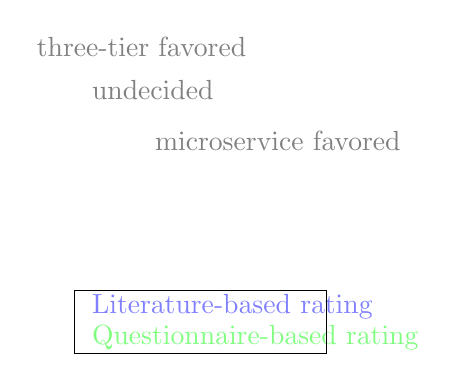
\begin{tikzpicture}
\tkzKiviatDiagram[scale=1.7,label space= 1.3, label distance=.1cm,
        radial  = 9,
        gap     = 1,  
        lattice = 3]{Resource efficiency with varying load, Horizontal scaling of components, Availability after component crash, Transaction consistency, Data consistency, Modifiability on \\ component level, Component reuse, Data segregation, Installability on premise}
\tkzKiviatLine[thick,color=blue,mark=none,
               fill=blue!20,opacity=.5](3,3,2,1,1,3,3,2,1)
\tkzKiviatLine[thick,color=darkgray,
               fill=green!20,opacity=.5](2.7,2.65,2.5,1.35,1.5,2.85,2.2,2.15,1.45) 
%\tkzKiviatLine[ultra thick,mark=ball,
%                 mark size=4pt,color =red](2,3.75,1,1.5,2)    
%\tkzKiviatGrad[prefix=,unity=1,suffix=](1)  
\node[color=gray, right] at (0.8,-0.7) {three-tier favored};
\node[color=gray, right] at (1.5,-1.25) {undecided};
\node[color=gray, right] at (2.3,-1.9) {microservice favored};
%legend
\node[color=blue!50, right] at (1.5,-4) {Literature-based rating};
\node[color=green!50, right] at (1.5,-4.4) {Questionnaire-based
 rating};
\draw (1.4, -3.8) -- (4.6, -3.8) -- (4.6, -4.6) -- (1.4, -4.6) -- (1.4, -3.8);
% Arrow
%\node (A) at (1.7, -5)[fill=black, draw,shape=circle, minimum size=0.2cm,inner sep=0]{};
%\node (B) at (4.3, -5)[]{};
%\draw [->] (A) edge (B);
%\node (C) at  (2.4, -5.2){};
%\node (D) at  (2.4, -4.8){};
%\draw [-] (C) edge (D)[color=gray];
%\node (E) at  (3.2, -5.2){};
%\node (F) at  (3.2, -4.8){};
%\draw [-] (E) edge (F)[color=gray]; 
%\node (G) at  (3.9, -5.2){};
%\node (H) at  (3.9, -4.8){};
%\draw [-] (G) edge (H)[color=gray]; 
\end{tikzpicture}
 \caption[KivatDiagram showing a graphical representation between literature and interview based evaluation regarding microservices and given quality scenarios]{Diagram showing a graphical representation of the results of literature based rating(blue) and interview based rating(green) regarding the question "How well are microservices suited to achieve the given quality scenario in comparison to a three-tier architecture". In total nine quality scenarios were evaluated. The graphic visualizes strong overlapping in the results between the two rating methods.}
\label{fig:kiviatQuality}
\end{figure}

A tabular representation of the data is listed in table \ref{res:table}.
The table shows literature and questionnaire-based rating.
All ratings are placed on a continuum between minus one and plus one.
It shows the relative rating for each scenario between microservices and three-tier architecture.
Again this refers to the question: Which architectural style is more suitable to achieve the given quality scenario.
Minus one stands for three-tier architecture favored, zero means undecided and plus one stands for microservice favored.

The difference column shows that the biggest outliers in rating show a difference of 0.8 and 0.5.
The outliers are going to be discussed in Section~\ref{res:discussion}.
The general tendency is that both methods produced strongly similar results.

\begin{table}[h]
  \renewcommand{\arraystretch}{1.2}
  \centering
  \sffamily
  \begin{footnotesize}
    \begin{tabular}{l l l l}
    \toprule
    \textbf{Quality attribute scenario} & \textbf{Literature-based rating} & \textbf{Questionnaire rating} & \textbf{Difference}\\
    \midrule
    Resource efficiency with varying load	&	1.0 	& 0.7 & 0.3\\
    Horizontal scaling of components	&	1.0		&	0.65  & 0.35\\
    Availability after component crash	&	0.0	&	0.5  & \textbf{0.5}\\
    Transaction consistency	&	-1.0		&	-0.65  & 0.35 \\
    Data consistency	&	-1.0		&	-0.5  & \textbf{0.5} \\
    Modifiability on component level	&	~1.0		&	0.85  & 0.15 \\    
    Component reuse	&	1.0		&	0.2  & \textbf{0.8} \\    
    Data segregation	&	0.0		&	0.15  & 0.15 \\    
    Installability on premise	&	-1.0		&	-0.55  & 0.45 \\                
    \bottomrule
    \end{tabular}
  \end{footnotesize}
  \rmfamily
  \caption[Quantified comparison between the literature and questionnaire-based evaluation.]{Quantified comparison between the literature and questionnaire-based evaluation. Negative one stands for three-tier architecture favored, zero means undecided and plus one stands for microservice favored. Differences larger or equal 0.5 in rating are highlighted in bold.}
  \label{res:table}
\end{table}


In conclusion, the results suggest that the evaluation of quality attribute scenarios done in Chapter~\ref{qua:qualitiesRating} based on literature research is backed up by the results of the questionnaire realized with microservice experts at SAP.

\clearpage

\subsection{Organizational qualities}

Four organizational requirements were evaluated by using literature-based research (see Section~\ref{quaMicro:tradeoffOrgRequirements}) and by using a questionnaire in regard to the question: ``Which architectural style (microservices or three-tier architecture) works better together with a given organizational requirement''.

Figure~\ref{fig:kiviatOrganizational} visualizes the results.
It shows the rating based on literature (blue) and the rating based on the questionnaire (green).
When looking at the overlapping of both quadrangles it becomes clear that both ratings share the same tendency regarding all four organizational requirements.

In detail the ratings show that:
\textit{Technical teams} and \textit{quality gates} strongly favor a three-tier architecture.
\textit{Explicit Interfaces} lightly and \textit{high development velocity} strongly favors microservices.
This is backed up by both literature as well as questionnaire based rating.

\begin{figure}
\centering
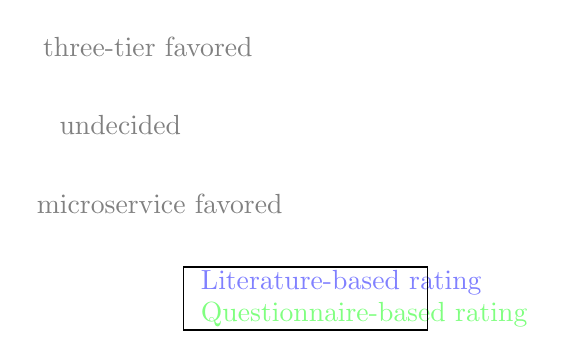
\begin{tikzpicture}
\tkzKiviatDiagram[scale=1.7,label space= 1.3, label distance=.1cm,
        radial  = 4,
        gap     = 1,  
        lattice = 3]{Technical teams, Explicit Interfaces, High development velocity, Quality gates}
\tkzKiviatLine[thick,color=blue,mark=none,
               fill=blue!20,opacity=.5](1,3,3,1)
\tkzKiviatLine[thick,color=darkgray,
               fill=green!20,opacity=.5](1.45,2.45,2.7, 1.55) 
\node[color=gray] at (0.95,-1) {three-tier favored};
\node[color=gray] at (0.6,-2) {undecided};
\node[color=gray] at (1.1,-3) {microservice favored};
%legend
\node[color=blue!50, right] at (1.5,-4) {Literature-based rating};
\node[color=green!50, right] at (1.5,-4.4) {Questionnaire-based rating};
\draw (1.4, -3.8) -- (4.5, -3.8) -- (4.5, -4.6) -- (1.4, -4.6) -- (1.4, -3.8);
\end{tikzpicture}
 \caption[KivatDiagram showing a graphical representation between literature and interview based evaluation regarding microservices and organizational requirements]{The diagram shows a graphical representation of the results of literature based rating(blue) and questionnaire based rating(green) regarding the question: "rate which architectural style (microservices and three-tier architecture) works better together with the given organizational requirement''. In total 4 organizational requirements were evaluated. The graphic again shows strong overlapping in the ratings between the two rating methods.}
\label{fig:kiviatOrganizational}
\end{figure}

\clearpage
\section{Discussion}
\label{res:discussion}
This section summarizes the interpretation of the results from the questionnaire.
The learnings reach beyond the pure numerical results.

\paragraph{Questionnaire results support literature-based evaluation}
The results of the questionnaire support the rating of the literature-based trade-off discussion from Chapter~\ref{qua:qualitiesRating}.
There were some outliers, like the scenarios \textit{component reuse}, \textit{data consistency} and \textit{availability after component crash}.
But even these are within a small margin and show the same tendency overall.

The biggest outliers were produced from the scenarios where the questionnaire participants engaged in conversation after the questionnaire. 
These scenarios left room for interpretation and different participants understood the scenarios differently.
This variance is partly reflected in the rating of these scenarios.
Especially regarding the \hyperref[quaMicro:s17]{scenario 17 - component reuse} participants were unsure about the type of component to be reused. 
The outliers are a pointer to the scenarios that might be formulated too vaguely and left room for interpretation. 

\paragraph{Application scenario rating failed}
Originally, the questionnaire was designed to match application scenarios with quality attributes.
The goal was do give a definitive guideline in which of the application scenarios to use microservices through an indirect mapping over quality attribute scenarios.
As elaborated in \ref{que:evalProcess} this approach failed.
This thesis suggests that the approach to match architectural styles with abstract application scenarios by rating quality attributes was flawed:

Firstly, if application scenarios are formulated in a rather general matter then it is hard to rate quality attributes for them at all. 
Different participants interpret the scenarios differently, which leads to unreliable results.

Secondly, company policies, team knowledge and other surrounding factors influence the decision for or against microservices strongly.
Therefore, it is hard to give a general advice with generally formulated application quality scenarios.
Even popular software architecture books, like \citep{Bass2012} do not recommend architectural styles for certain application types. 
The real world is just more complex than what an abstracted evaluation can conceive.

\paragraph{Researching the obvious}
In the questionnaire the participants were asked to rate 9 architectural qualities and 4 organizational requirements with regard to how well they fit together with microservices.
The presented architectural and organizational qualities mostly relate to the obvious and popularized qualities and disadvantages of microservices.
Supposedly without surprise, the results of the questionnaire support the evaluation done in the literature-based evaluation.

Did the questionnaire surface something unexpected? Probably, not.
Does this mean the questionnaire had no merit to it? No, it definitely had merit and that on different levels:

First of all, while it was probable, it was by no means certain that the questionnaires results will support the literature based evaluation.
In the end supporting arguments with different, unrelated sources makes them stronger.
This especially applies to a new concept like microservices, where the literature might not be as settled and approved as in other fields.
 
 %TODO small sample size could also explain
Secondly, while the answers in the questionnaire in general supported the evaluation there still were some interesting differences.
For example, regarding the component reuse scenario \hyperref[quaMicro:s17]{17} the standard deviation was 0.55, which is the highest value of derivation in the sample. 
That means that the amount of spread or distance from the mean is 0.55 when values between zero and two could be selected.
It seems that this topic is heavily discussed and the practitioners mostly disagree with each other whether microservices are better reusable than components in a three-tier architecture. 
This is an interesting observation as also literature writes very sparely on the reuse of microservices.

Thirdly and most importantly, the sophisticated discussion with participants about the questionnaire surfaced a general problem of this kind of architectural evaluation:
\begin{itemize}
\item Architectural trade-offs in real projects are much more complex than broad, general quality scenarios are able to express. Quality attribute scenarios seem to mainly have value if they are connected to a concrete use case.
\item The decision for an architectural style is dependent on much more than just quality attributes of the application. Factors like team knowledge, company organization and project size influence the architectural decisions heavily.
\end{itemize}

In conclusion a general architectural decision guidance cannot be provided purely on the basis of quality scenarios.
Every use case is different and though must be discussed individually.
The trade-off discussion in Chapter~\ref{qua:qualitiesRating} is a discussion starter for that.
\chapter{Conclusion}
\label{con}
%TODO a little to retrospective

\section{Summary}
Prior work on the topic of the microservice architectural style mainly covers general overviews \cite{Newman2015,Wolff2016}. 
As there is no common definition of the relatively new term microservices, different sources draw different, coarse pictures of its characteristics.
Many refer to the successful flagship implementations in the industry, like Netflix or Amazon.
But, there is no thorough trade-off discussion of microservices, as well as no explicit decision guidance for which application scenarios to use microservices known to the author of the thesis.

The thesis used quality attribute scenarios to systematically discuss trade-offs of microservices.
A list of quality scenarios relevant for the evaluation of microservices was created (Section~\ref{qua:architecturalQua}).
Each quality scenario was assessed and discussed in regard to whether microservice or the three-tier architectural style is more suitable to achieve the scenario (Section~\ref{quaMicro:rating}).
In addition, organizational factors and their influence on using microservices were discussed (Section~\ref{quaMicro:tradeoffOrgRequirements}).
This evaluation was based on research from literature, conference talks and analysis of industry examples of microservice architectures. 
A subset of the scenarios was empirically evaluated by interviewing microservice practitioners through a questionnaire (Chapter~\ref{que:empiricalEvaluation}).

During the evaluation of the quality attributes it became clear that giving a general guidance in which application scenarios to use microservices cannot be achieved by this thesis.
Firstly, a high-level description of an application scenario is too vague to be reliably assessed regarding quality attributes. 
Secondly, the decision which architectural style to use is dependent on many factors (quality attributes are just one of them) and they cannot all be covered here.
% in order to give a realistic decision guidance.
Trade-offs on several layers contribute to the decision of using microservices or not.

However, what this thesis presents is a discussion of different trade-offs of microservices in comparison to more monolithic styles, like a three-tier architecture.
Not a definite decision guideline, but a discussion starter is presented based on the condensed knowledge of several microservice practitioners.
In addition to quality attributes, also organizational factors are discussed, which play a major role in the decision for or against microservices.

Summarizing the findings from the quality rating in Section~\ref{quaRating:conclusion} microservices should be considered for the following use cases (related quality scenario numbers in brackets):

\begin{itemize}
\item High development velocity, meaning continuous innovation in large projects consisting of several teams (\hyperref[quaMicro:s16]{16} and organizational scenarios \hyperref[quaMicro:so1]{1}, \hyperref[quaMicro:so2]{2}).
\item High availability for large scale distributed systems, especially if eventual consistency can be accepted (\hyperref[quaMicro:s12]{12}, \hyperref[quaMicro:s13]{13}).
\item Excellent utilization of on-demand hardware through fine-grained auto-scaling of load. For example \textit{pay for service} (\hyperref[quaMicro:s2]{2}, \hyperref[quaMicro:s4]{4}, \hyperref[quaMicro:s22]{22}). 
\end{itemize}

On the contrary, one should rather not consider microservices if:

\begin{itemize}
\item The domain of the project is not fully known (see \textit{\hyperref[quaMicro:modifiabilityDiscussion]{modifiability discussion}} in \ref{quaMicro:modifiabilityDiscussion}).
\item The organization does not have or is not ready to heavily invest in competence to develop and operate complex, distributed systems (\hyperref[quaMicro:s9]{9}, \hyperref[quaMicro:s10]{10} and see \textit{\hyperref[quaMicro:distributedSystemDownsides]{distributed system discussion}} in \ref{quaMicro:distributedSystemDownsides}).
\item ACID conform transactions spanning over multiple business areas are needed (\hyperref[quaMicro:s11]{11}).
\end{itemize}

For most other quality attributes, microservices in comparison to three-tier architectures have up- and downsides.
Section~\ref{quaMicro:distributedSystemDownsides} holds a discussion of these trade-offs ordered by quality attributes.
An empirical evaluation through a questionnaire support the results of this evaluation (Section~\ref{res:overview}).

\section{Outlook and future work}
Microservices are another tool in the architectural toolkit that need to be chosen appropriately.
They will not replace monolithic applications in the near future.
Instead, they present themselves as an alternative to other architectural styles.
To conclude the thesis, this section discusses promising fields for future work on microservices.

\paragraph{Adoption of microservices}
At this moment it is too early to provide a final judgment of how effective microservices actually are. 
Most microservices applications are still rather young and how modifiable a system is will be evident after years.
As Fowler states, it is likely that the success of microservices is dependent on many factors in the surrounding environment, both political and technological \cite{FowlerMSOverview}.
For example, the skill of developers to handle the challenges of a distributed system might play an important role in how successful the style will be in a concrete use case.

Because most microservices-based applications are still rather young this thesis comes with a caveat. 
It uses information from the early adopters of microservices, which are probably not representative for all companies.
Only the future will tell whether the later adopters will be successful with microservices.
This will decide whether microservices can emerge from being a hyped topic to becoming an established and widely adopted architectural style.
Future work will have to constantly validate the currently known trade-offs of microservices with the growing evidence coming from teams sharing their experiences.
Also researching anti-patterns from failed microservice adoptions would be interesting.

\paragraph{Organizational implications of microservices}
This thesis offers a glimpse on the organizational implications of microservices.
Apparently, system design is inherently connected with the organizational structure of a company \citep[p. 201]{Newman2015}.
For example, microservices are frequently associated with the inverse Conway Maneuver (for Conways Law see \ref{bac:organisationalCharacteristics}).
The idea is to let the system design influence the team structure, instead of the other way around \citep[p. 201]{Newman2015}.
For microservices, this would mean that the teams follow the separation of services into business capabilities.
Reorganizing teams in an established organization into small independent teams is a large investment and future work could give examples and provide support on how to do that.

Another team related concept touched in this thesis is cross-functional teams.
Following the Amazon.com example, a microservice should be built and operated by one single team.
This team is ``completely responsible for the service -- from scoping out the functionality, to architecting it, to building it, and operating it \cite{Vogels2006}''.
This underlines the point that the decision for microservices has implications for team structure and organization.
It seems that a discussion about the organizational implications of microservices is underrepresented in the current literature, especially in relation to its importance.
Further researching the organizational implications of microservices seems to be interesting and highly relevant.

\paragraph{Patterns and strategies for implementing microservices}
With microservices, the complexity rises in fields like operation, deployment or programming.
The fact that microservices decouple the lifecycles of components enables innovation but acts as a complexity booster \cite{FowlerTradeoffsDistribution2015}.
Certain patterns and strategies are described as de facto standards for microservice architectures.
A few of them are:
\begin{itemize}
\item Tactics for reliability, like Bulkhead
\item Automated deployment with \ac{CD} and automated infrastructure provisioning
\item Sophisticated monitoring and logging setups
\item Simulating failure in production
\item Service interface versioning strategies
\item Patterns to implement network communication between services
\item Strategies to deal with partial failures and indeterminacy in a distributed system \cite{Kendall1994}.
\end{itemize}
These strategies did not necessarily evolve with microservices but they are inherently important for them, or arguably any large scale distributed system.
An approach that researches these strategies and patterns in order to give concrete guidance on how to handle the complexity and challenges of microservices appears useful and promising.

% Kerniger Schlusssaz, ein kerniges Statement zu meinen Erkenntnissen und oder was weitere Forschung hinzufügen kann.

% ------------------------------------------------------------------

\label{lastpage}

% Neue Seite
\cleardoublepage

% Backmatter mit normalem Zeilenabstand setzen
\singlespacing

% Römische Ziffern für die "Back-Matter", fortlaufend mit "Front-Matter"
\pagenumbering{roman}
\setcounter{page}{\value{frontmatterpage}}

% List of abbreviations
\chapter*{List of abbreviations}
\addcontentsline{toc}{chapter}{List of abbreviations}

\begin{acronym}
\acro{API}{Application Programming Interface}
\acro{AWS}{Amazon Web Services}
\acro{BBS}{Bulletin Board System}
\acro{CAPI}{Common Application Programmer's Interface}
\acro{CD}{Continuous Delivery}
\acro{CI}{Continuous Integration}
\acro{DDD}{Domain Driven Design}
\acro{GCP}{Google Cloud Platform}
\acro{& }{Graphical User Interface}
\acro{HA}{high availability}
\acro{HTTP}{Hypertext Transfer Protocol}
\acro{IaaS}{Infrastructure as a Service}
\acro{IEEE}{Institute of Electrical and Electronics Engineers}
\acro{ISO}{International Organization for Standardization}
\acro{IEC}{International Electrotechnical Commission}
\acro{NIST}{National Institute of Standards and Technology}
\acro{OS}{operating system}
\acro{REST}{Representational State Transfer}
\acro{PaaS}{Platform as a Service}
\acro{RPI}{Remote Procedure Invocation}
\acro{SaaS}{Software as a Service}
\acro{SOA}{Service Oriented Architecture}
\acro{SQuaRE}{Software product Quality Requirements and Evaluation}
\acro{UAA}{User Account and Authentication}
\acro{UI}{User Interface}
\acro{URI}{Uniform Resource Identifier}
\acro{VM}{Virtual Machine}
\end{acronym}


% Tabellenverzeichnis erzeugen
\cleardoublepage
\phantomsection
\addcontentsline{toc}{chapter}{List of tables}
\listoftables

% Abbildungsverzeichnis erzeugen
\cleardoublepage
\phantomsection
\addcontentsline{toc}{chapter}{List of figures}
\listoffigures

% Listingverzeichnis erzeugen
%\cleardoublepage
%\phantomsection
%\addcontentsline{toc}{chapter}{List of sourcecode}
%\lstlistoflistings

% Protocol:
% First I changed bibliogrpahystyle from dinat to alpha because multiple authors were connect with "und" not "and". Then I received: Package natbib Error: Bibliography not compatible with author-year citations. 
% I found the solution by a) making sure all my bib entries had years and b) changing  square to numbers. This could be made the default behaviour for english work..
%\usepackage[square]{natbib}       % Literaturverzeichnis nach DIN mit eckigen Klammern bei \citep
%\usepackage[numbers]{natbib}

% Literaturverzeichnis erzeugen (nach DIN)
\begin{flushleft}
%\bibliographystyle{dinat} % Literatur nach DIN
%\bibliographystyle{abbrv} % Zitate mit [1], [2] etc.
\bibliographystyle{alpha} % Zitate mit [Kor01], [Vix99] etc.
\bibliography{literature}   % BibTeX-Datei mit Literaturquellen einbinden
\end{flushleft}

% Appendix erzeugen
%\cleardoublepage
%\begin{appendices}

%\end{appendices}

% Index ausgeben
\cleardoublepage
\phantomsection
\addcontentsline{toc}{chapter}{Index}
\printindex

\appendix
\chapter{Questionnaire}
\label{app:questionnaire}
\includepdf[pages={-}]{pdf/questionnaire.pdf}

\end{document}